%        File: technology.tex
%     Created: Sun Mar 31 03:00 PM 2013 C
% Last Change: Sun Mar 31 03:00 PM 2013 C
%


%\documentclass[11pt,handout]{beamer}
\documentclass[9pt]{beamer}
\usetheme[white]{Wisconsin}
%\title[short title]{long title}
\title[Geologic Repositories and the Fuel Cycle]{Geologic Repositories and the Fuel Cycle}
%\subtitle[short subtitle]{long subtitle}
\subtitle[NPRE412]{NPRE412}
%\author[short name]{long name}
\author[Kathryn D. Huff]{Kathryn D. Huff}
%\date[short date]{long date}
\date[10.31.2016]{October 31, 2016}
%\institution[short name]{long name}
\institute[UIUC]{University of Illinois at Urbana-Champaign}

%\usepackage{bbding}
\usepackage{amsfonts}
\usepackage{amsmath}
\usepackage{graphicx}
\usepackage{subfigure}
\usepackage{booktabs} % nice rules for tables
\usepackage{microtype} % if using PDF
\usepackage{bigints}
\newcommand{\units}[1] {\:\text{#1}}%
\newcommand{\SN}{S$_N$}%{S$_\text{N}$}%{$S_N$}%
\DeclareMathOperator{\erf}{erf}

%page numbers
\setbeamertemplate{footline}[page number]
%Those icons in the references are terrible looking
\setbeamertemplate{bibliography item}[text]
\begin{document}
%%%%%%%%%%%%%%%%%%%%%%%%%%%%%%%%%%%%%%%%%%%%%%%%%%%%%%%%%%%%%
%% From uw-beamer Here's a handy bit of code to place at 
%% the beginning of your presentation (after \begin{document}):
\newcommand*{\alphabet}{ABCDEFGHIJKLMNOPQRSTUVWXYZabcdefghijklmnopqrstuvwxyz}
\newlength{\highlightheight}
\newlength{\highlightdepth}
\newlength{\highlightmargin}
\setlength{\highlightmargin}{2pt}
\settoheight{\highlightheight}{\alphabet}
\settodepth{\highlightdepth}{\alphabet}
\addtolength{\highlightheight}{\highlightmargin}
\addtolength{\highlightdepth}{\highlightmargin}
\addtolength{\highlightheight}{\highlightdepth}
\newcommand*{\Highlight}{\rlap{\textcolor{HighlightBackground}{\rule[-\highlightdepth]{\linewidth}{\highlightheight}}}}
%%%%%%%%%%%%%%%%%%%%%%%%%%%%%%%%%%%%%%%%%%%%%%%%%%%%%%%%%%%%%
%%--------------------------------%%
\frame{
  \titlepage
}

\section{Geologic Repository Concepts}
%%--------------------------------%%
\begin{frame}
  \frametitle{Outline}
  \tableofcontents[currentsection]
\end{frame}

\subsection{Components}


%%----------------------------------------%%
\begin{frame}
  \frametitle{Repository Components}
\footnotesize{
  \begin{figure}[htbp!]
  \begin{center}
    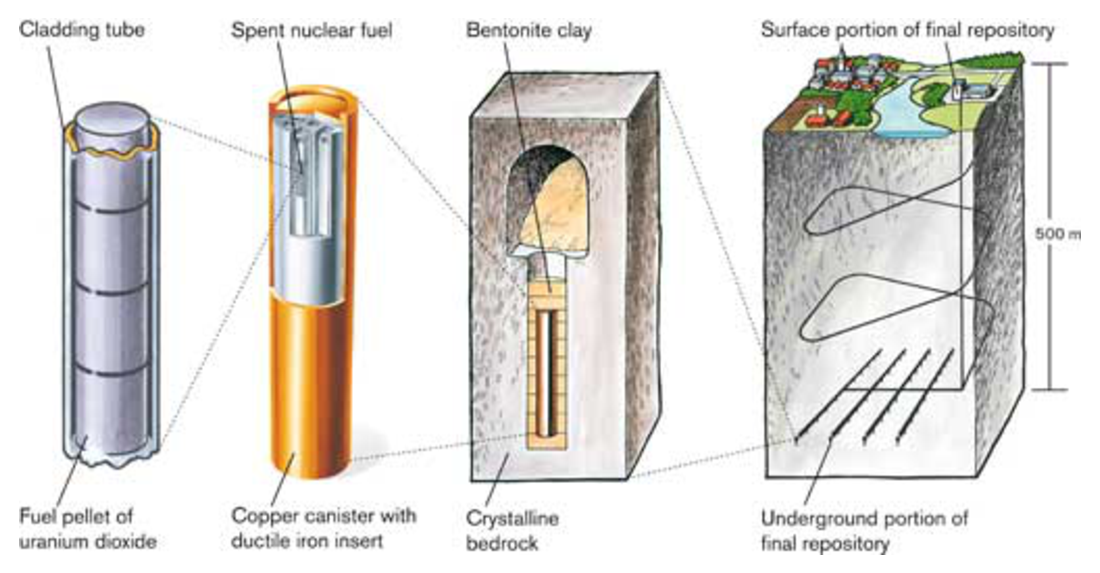
\includegraphics[width=0.7\textwidth]{./images/skb_components.eps}
  \end{center}
  \caption{Geologic disposal systems typically employ engineered barrier 
    systems as well as natural barrier systems. This is a Swedish concept in 
    granite \cite{ab_long-term_2006}.}
  \label{fig:skb_components}
\end{figure}

}
\end{frame}


\subsection{Layouts}
\begin{frame}
  \frametitle{Repository Layouts}

  \begin{minipage}{0.49\textwidth}
    \begin{figure}[h!]
      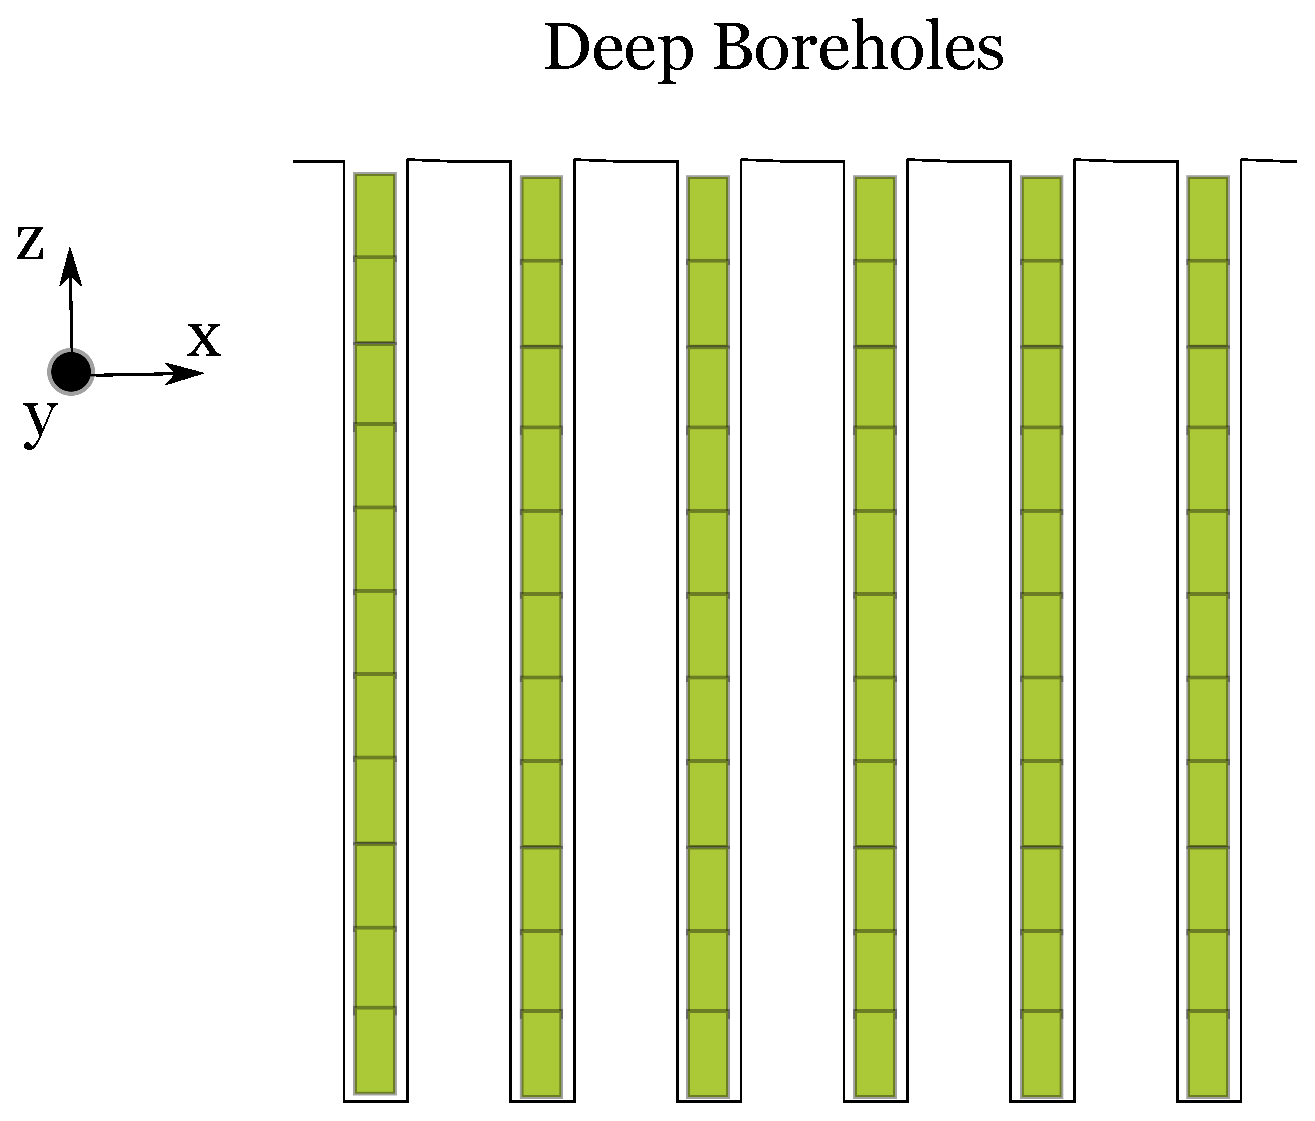
\includegraphics[width=0.75\textwidth]{./images/boreholes.eps}
    \end{figure}
    \begin{figure}[h!]
      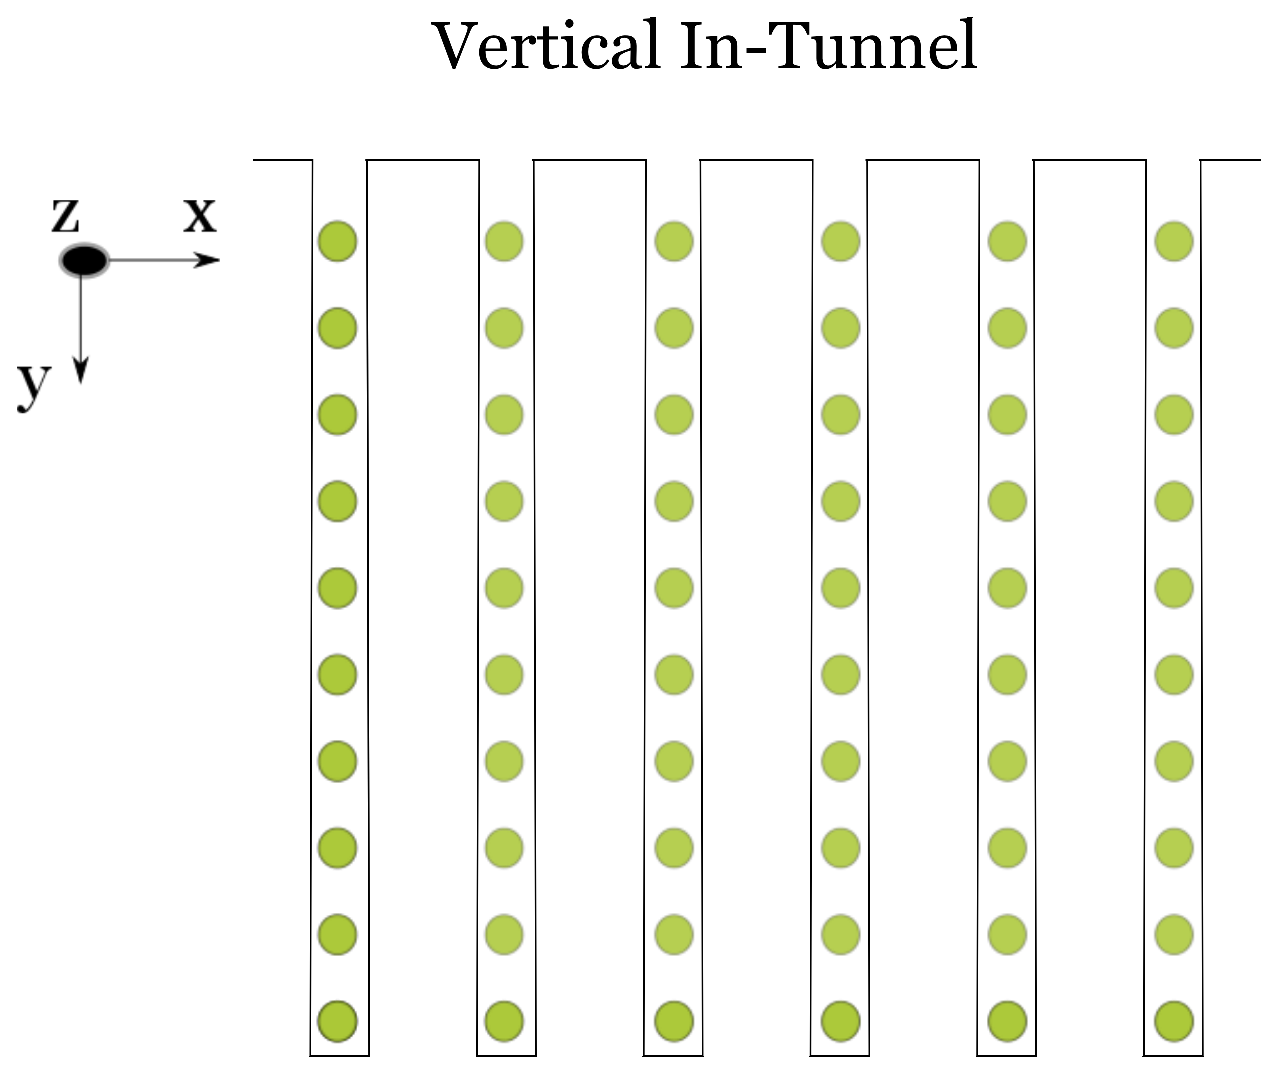
\includegraphics[width=0.75\textwidth]{./images/vertical.eps}
    \end{figure}
  \end{minipage}
  \hspace{0.01cm}
  \begin{minipage}{0.49\textwidth}
    \begin{figure}[h!]
      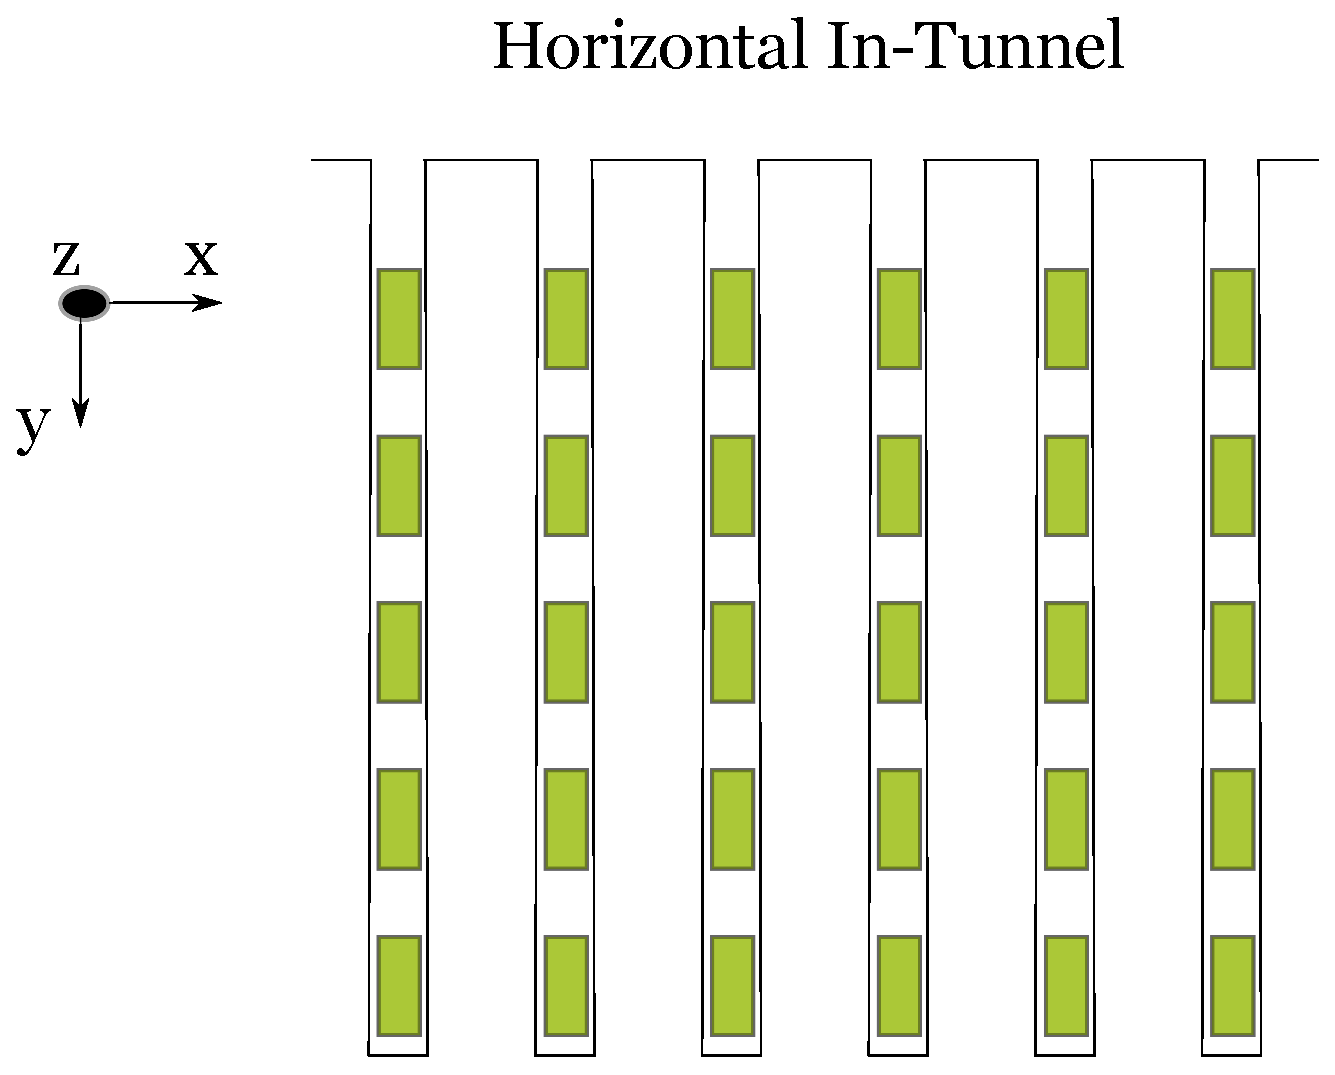
\includegraphics[width=0.8\textwidth]{./images/horizontal.eps}
    \end{figure}
    \begin{figure}[h!]
      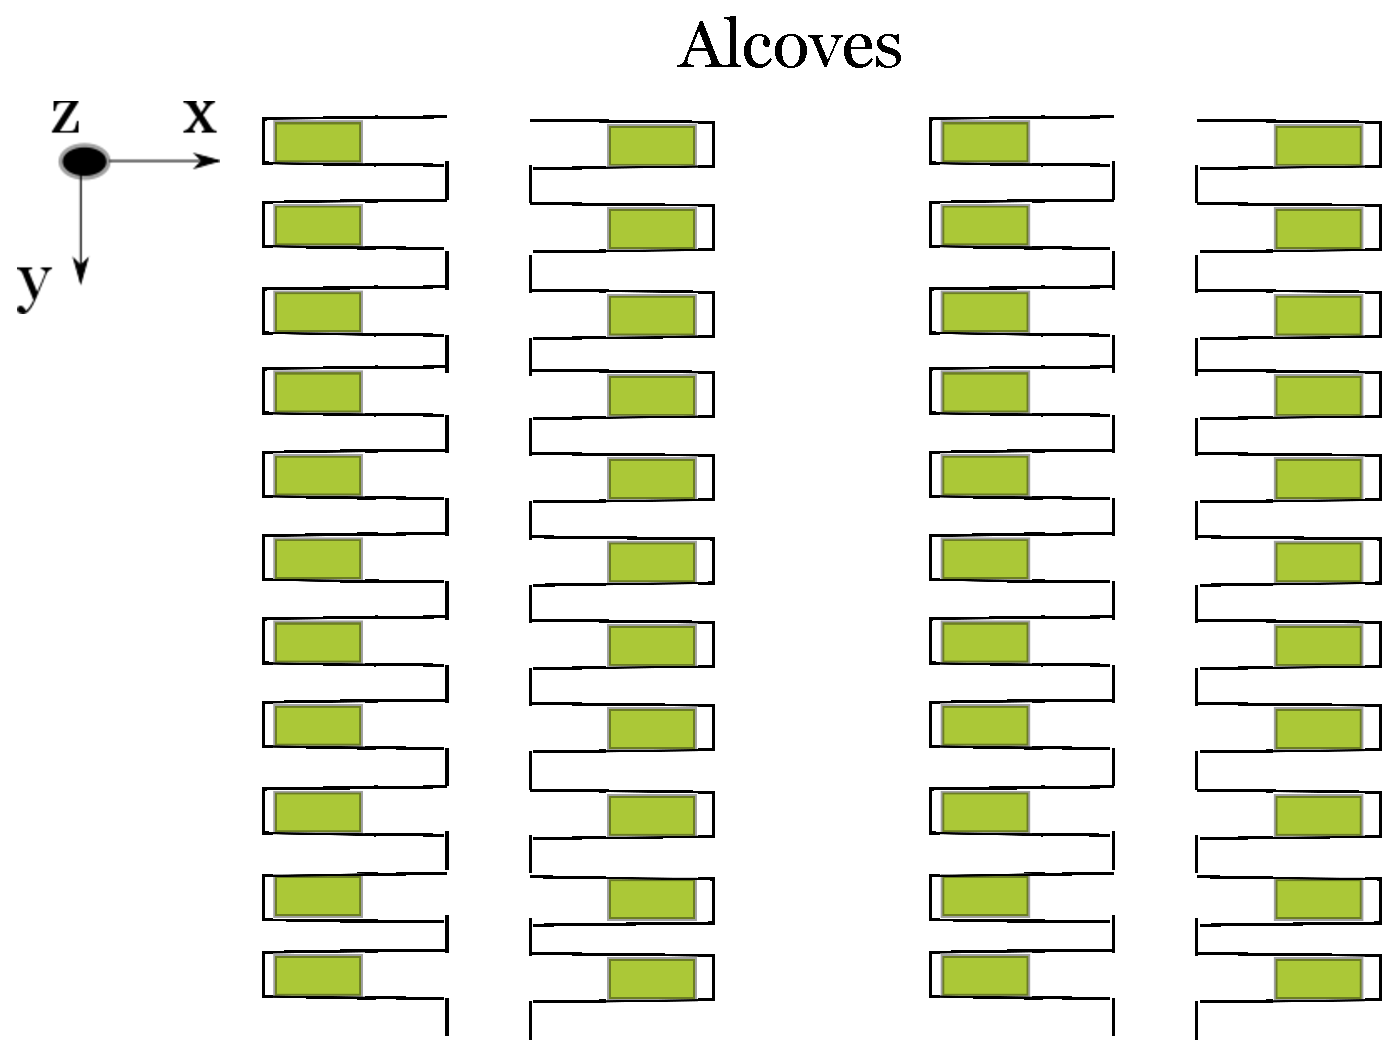
\includegraphics[width=0.8\textwidth]{./images/alcoves.eps}
    \end{figure}
  \end{minipage}

\end{frame}

\begin{frame}
  \footnotesize{
  \frametitle{Unsaturated, Ventilated Concepts}
  \begin{figure}[htbp!]
  \begin{center}
    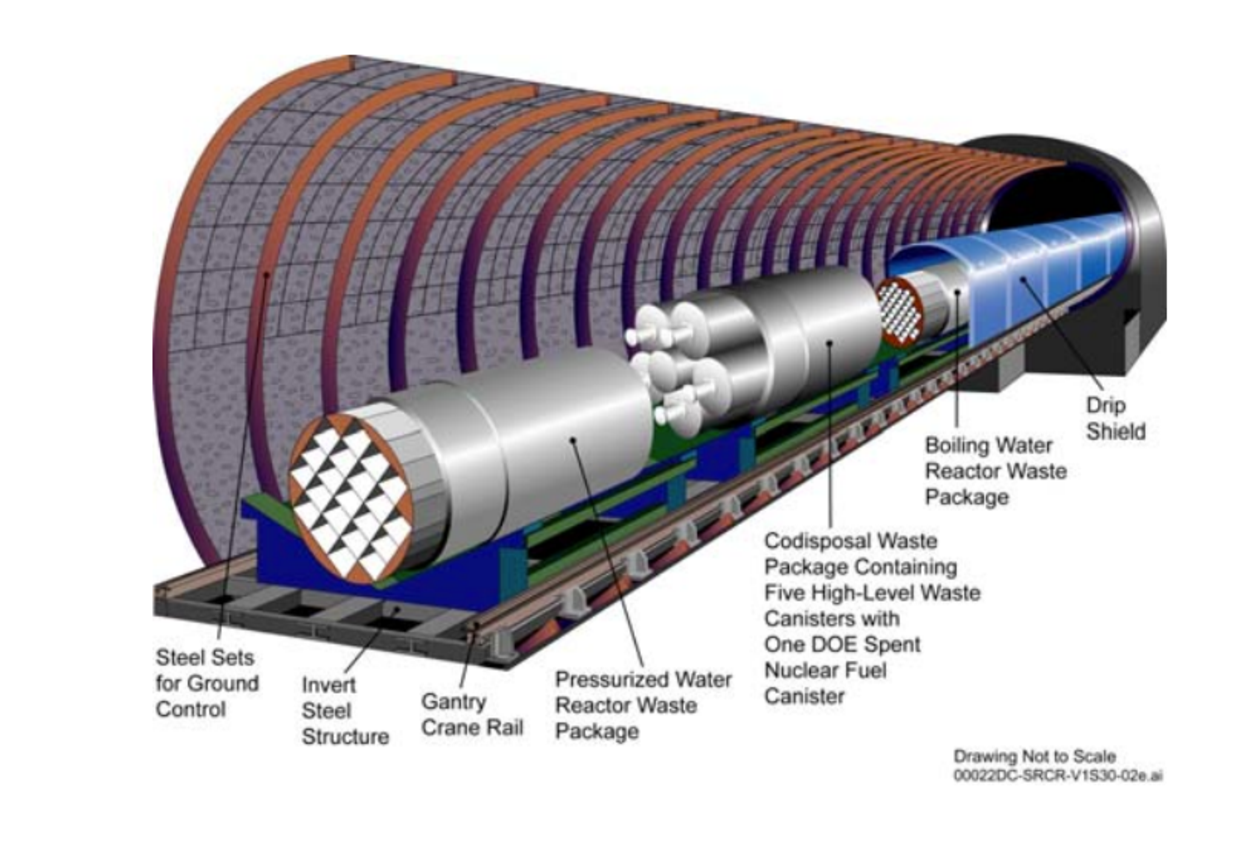
\includegraphics[height=0.7\textwidth]{./images/yucca_tunnel.eps}
  \end{center}
  \caption{The current U.S. geologic disposal concept \cite{peters_whats_2013}.}
  \label{fig:yucca_tunnel}
\end{figure}

}
\end{frame}

\begin{frame}
  \footnotesize{
  \frametitle{Saturated , Enclosed Concepts} 
 \begin{figure}[h!]
    \begin{center}
      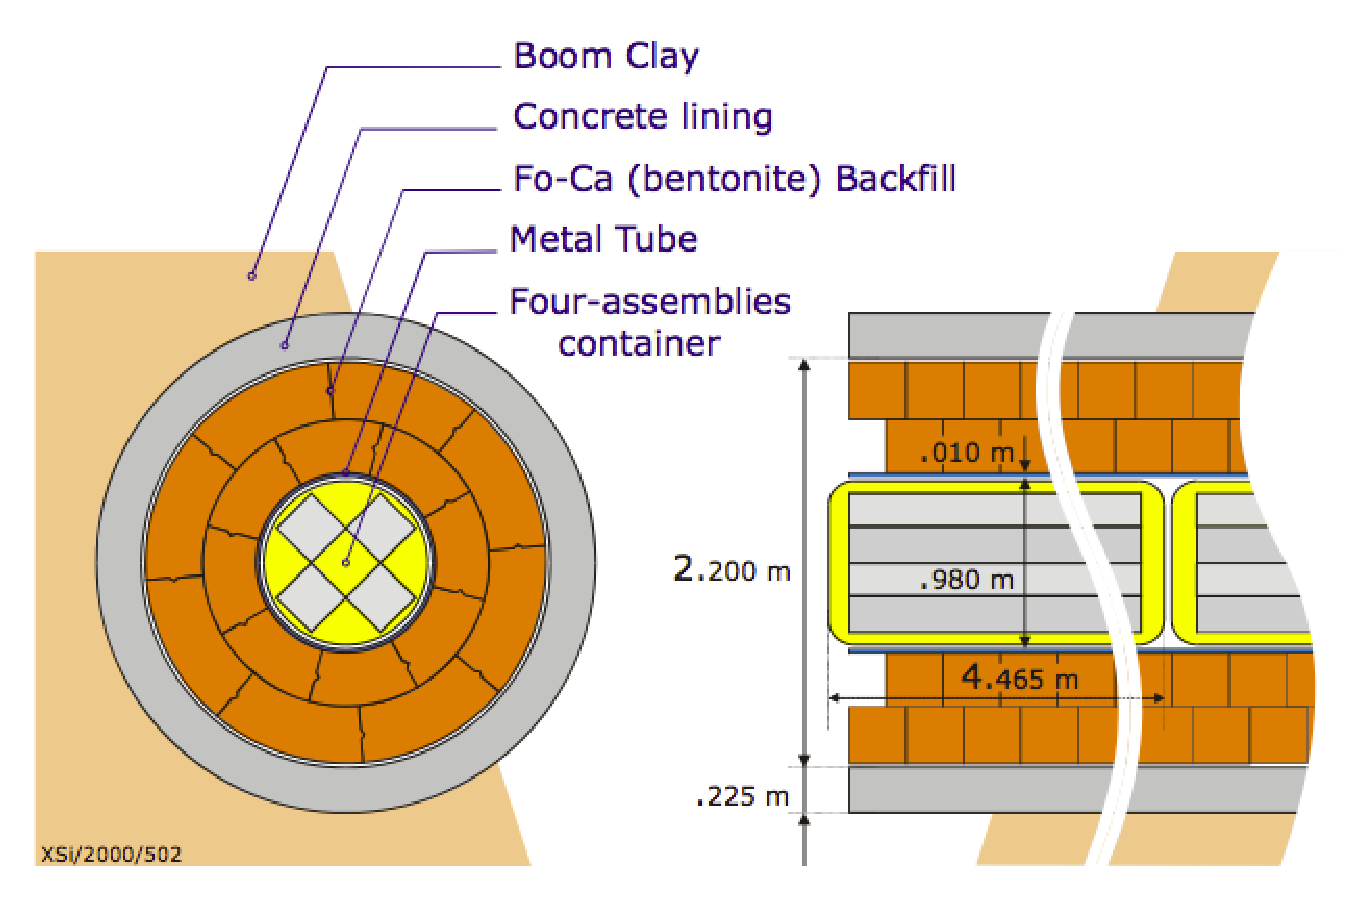
\includegraphics[height=.7\textheight]{./images/belgianClayRedImp.eps}
    \end{center}
    \caption{The Belgian reference concept in Boom Clay is backfilled very soon
   after waste emplacement without a ventilation period and is located below the water table
   \cite{von_lensa_red-impact_2008}.}
    \label{fig:belgianClayRedImp}
  \end{figure}
}
\end{frame}

\subsection{Geologies}


\begin{frame}
  \frametitle{Tuff (Yucca) Disposal Environments}
  \footnotesize{
    \begin{figure}[htbp!]
  \begin{center}
    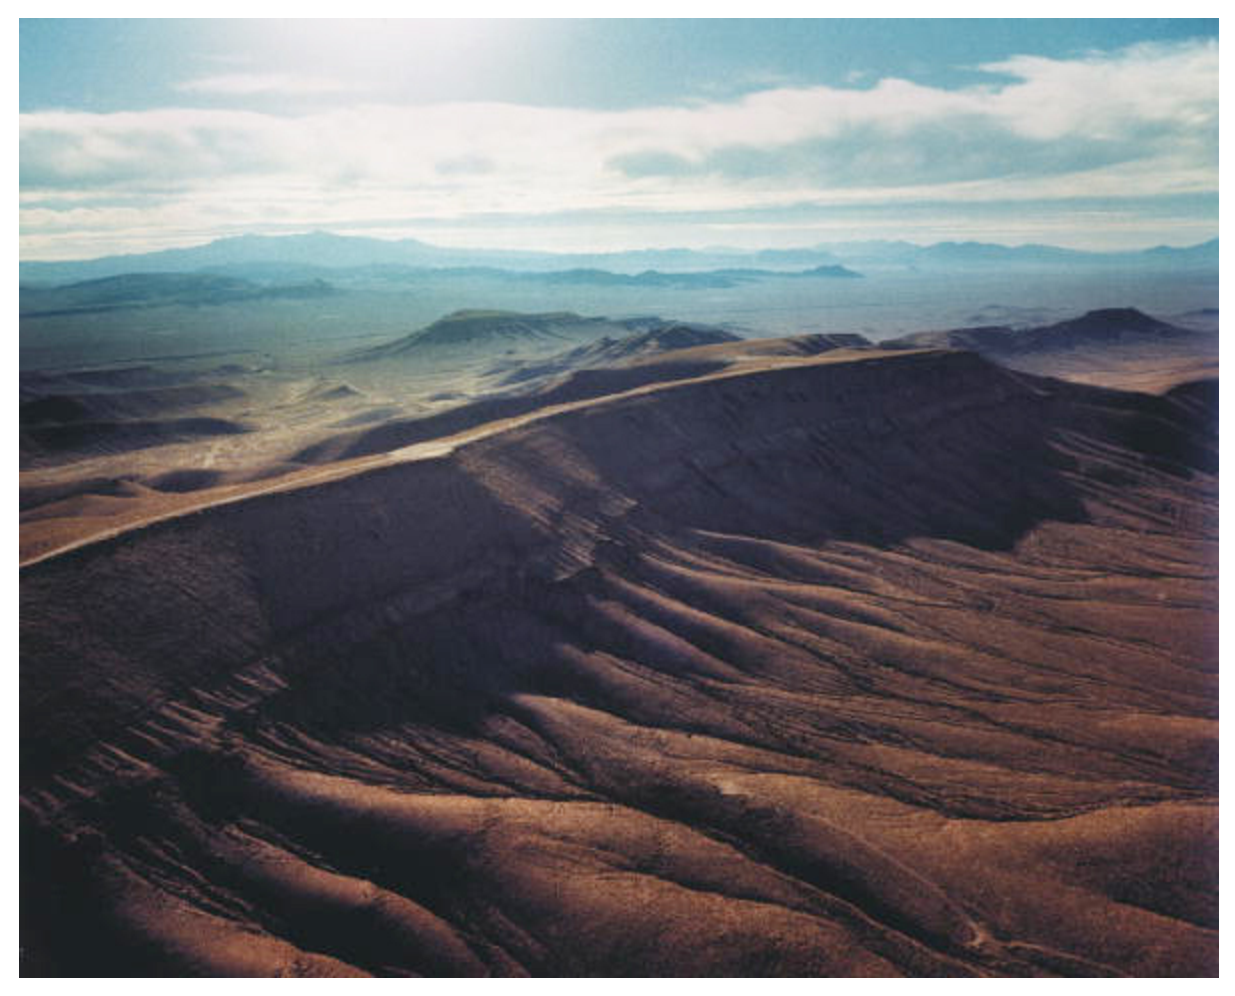
\includegraphics[width=0.5\textwidth]{./images/yucca_site.eps}
  \end{center}
  \caption{Yucca Mountain is in southern Nevada \cite{omb_yucca_2006}.}
  \label{fig:yucca_site}
\end{figure}

  }
\end{frame}

\begin{frame}
  \frametitle{Alternative Disposal Geology Options}
   \begin{minipage}{0.44\textwidth}
     \begin{figure}[h!]
         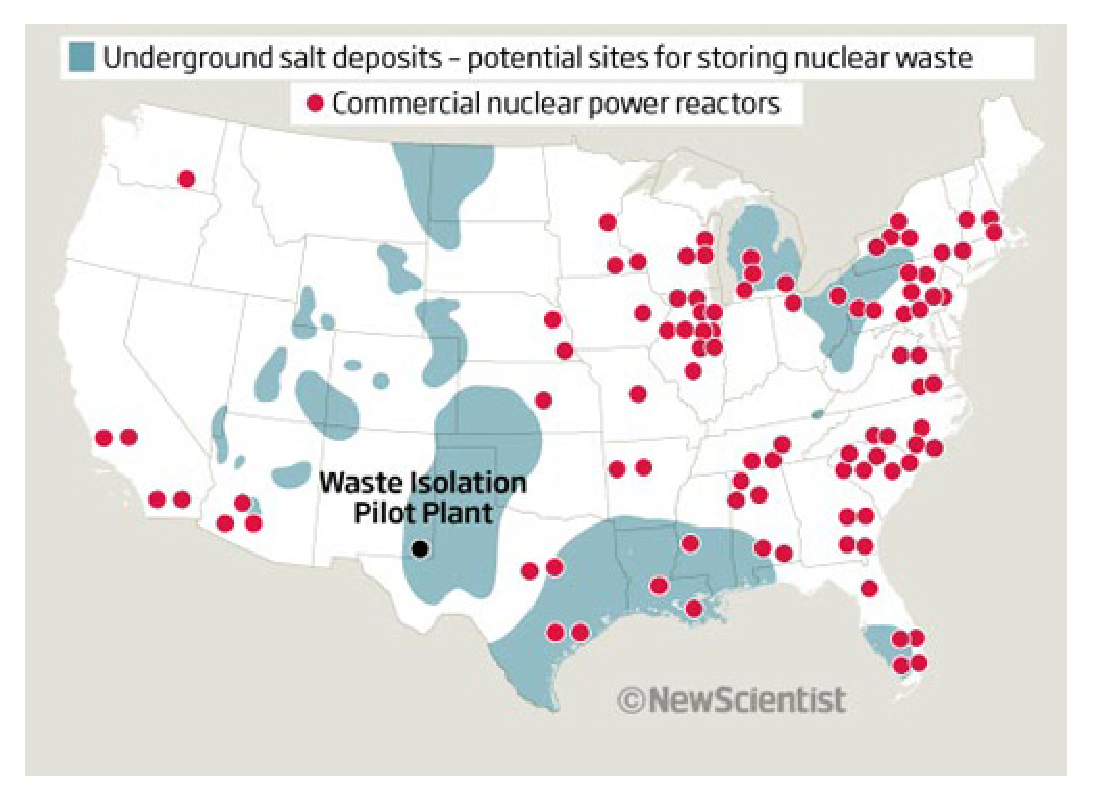
\includegraphics[width=0.8\textwidth]{./images/saltNewScientist.eps}
         \caption{U.S. Salt Deposits, ref. \cite{newscientist_where_2011}.}
     \end{figure}
     \begin{figure}[h!]
         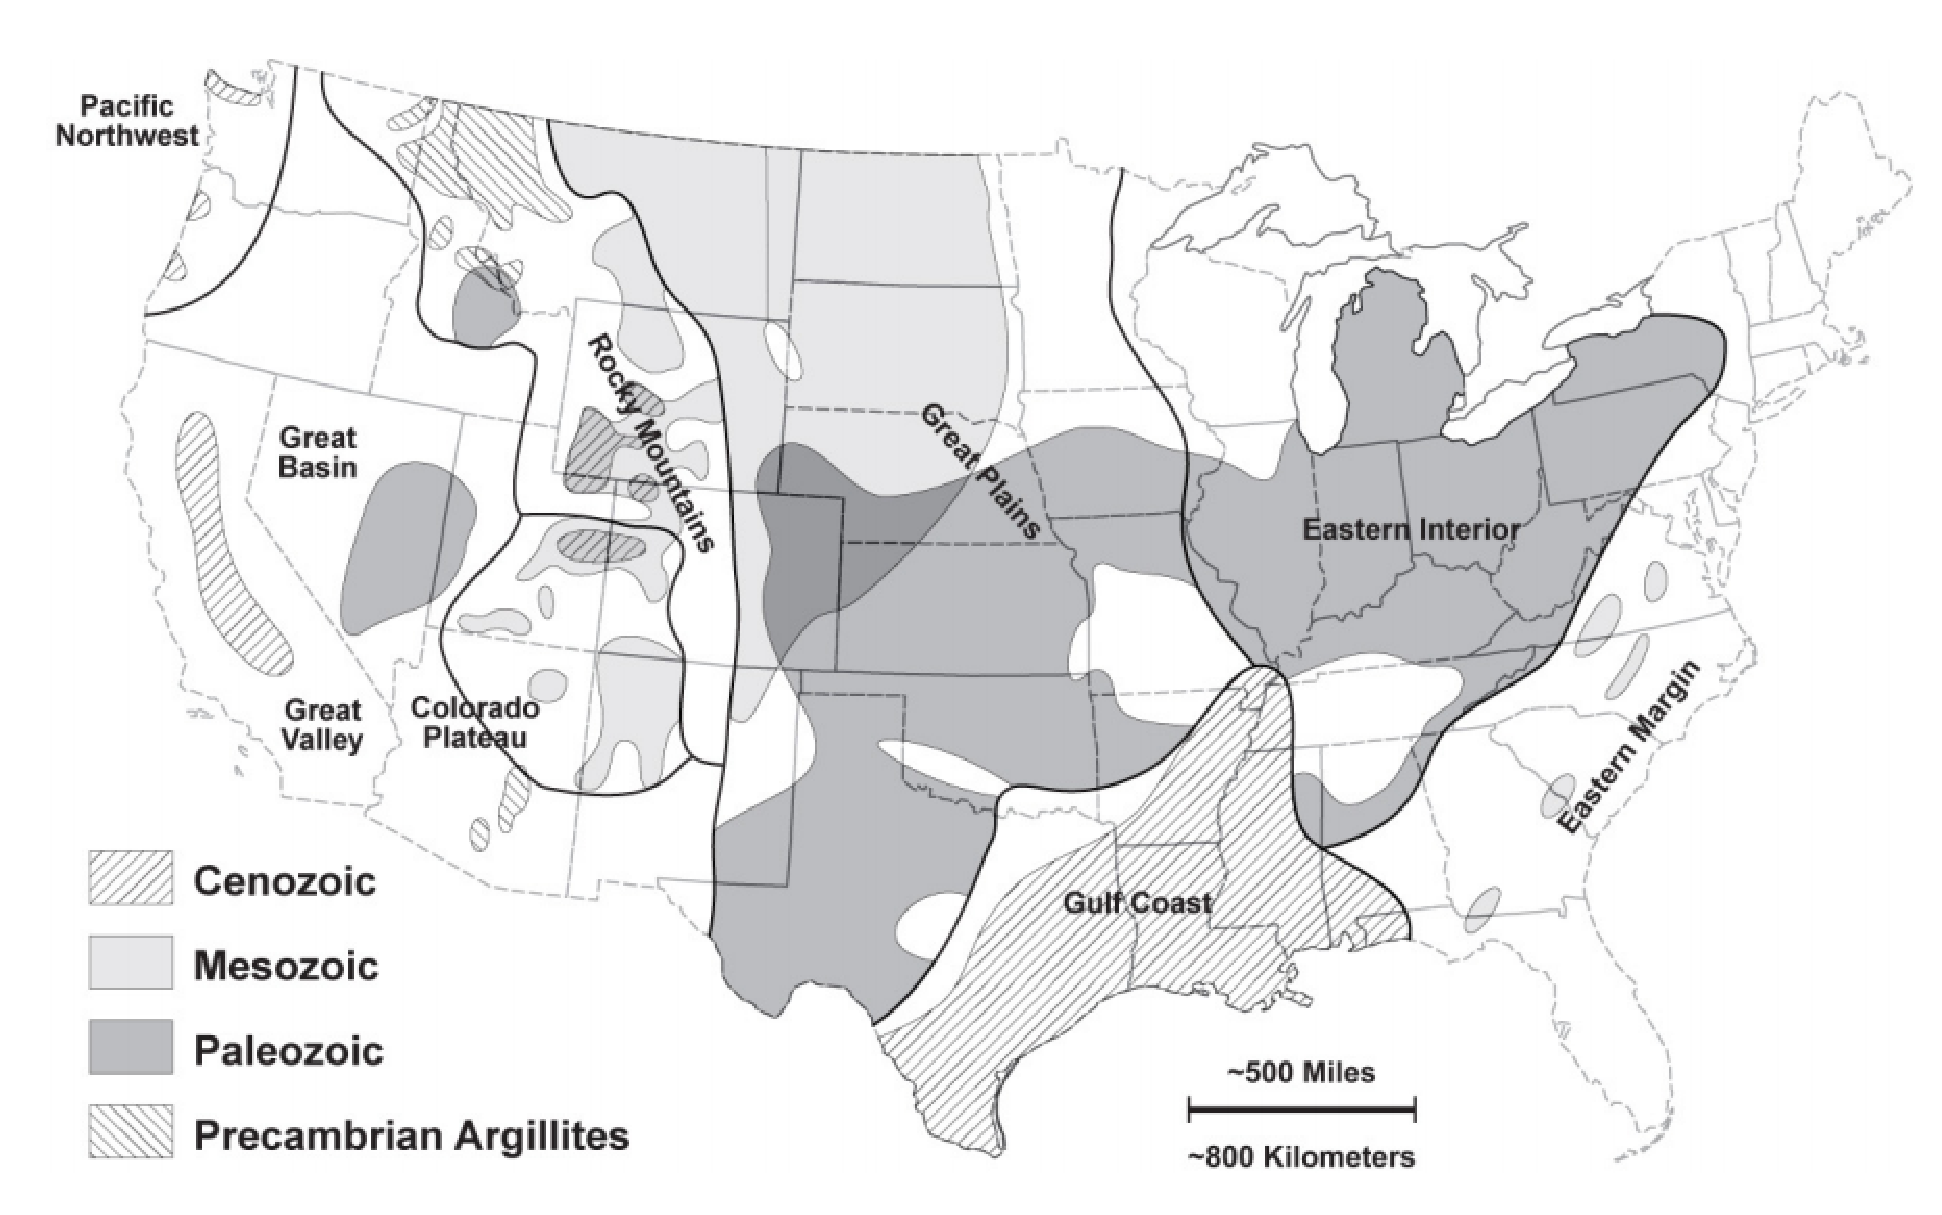
\includegraphics[width=0.8\textwidth]{./images/clayGonzales.eps}
         \caption{U.S. Clay Deposits, ref. \cite{gonzales_shales_1985}.}
     \end{figure}
   \end{minipage}
   \hspace{0.01cm}
   \begin{minipage}{0.44\textwidth}
     \begin{figure}[h!]
         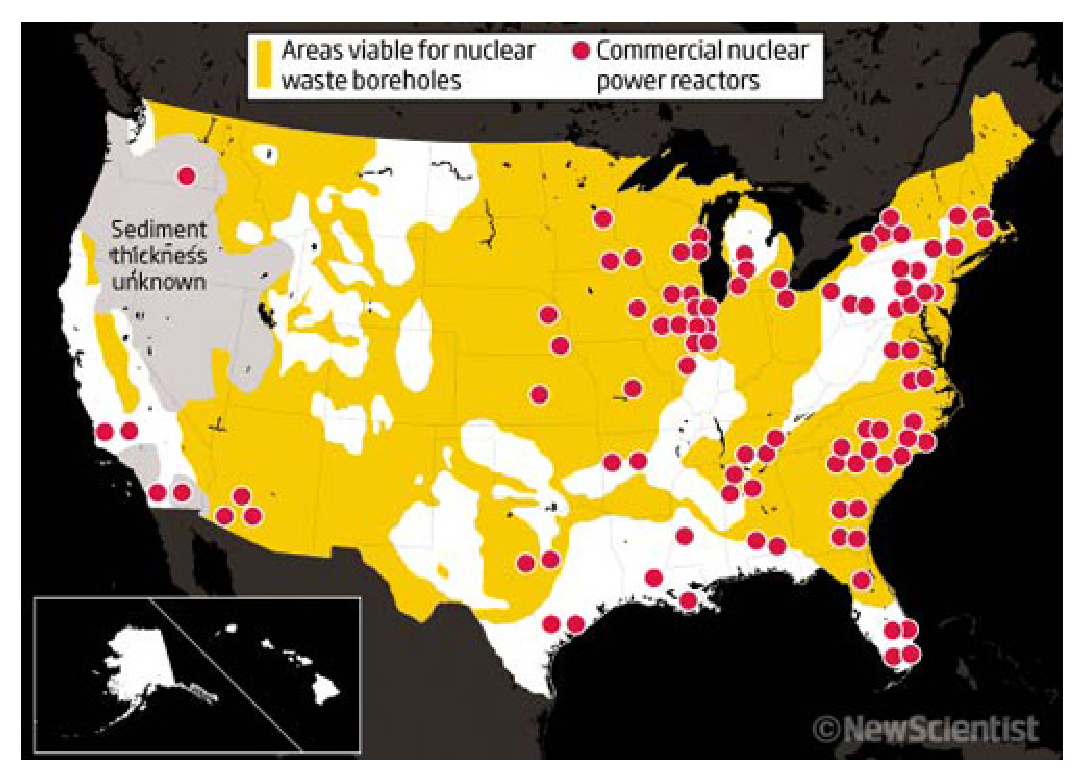
\includegraphics[width=0.8\textwidth]{./images/boreholeNewScientist.eps}
         \caption{U.S. Crystalline Basement, ref.  \cite{newscientist_where_2011}.}
     \end{figure}
     \begin{figure}[h!]
         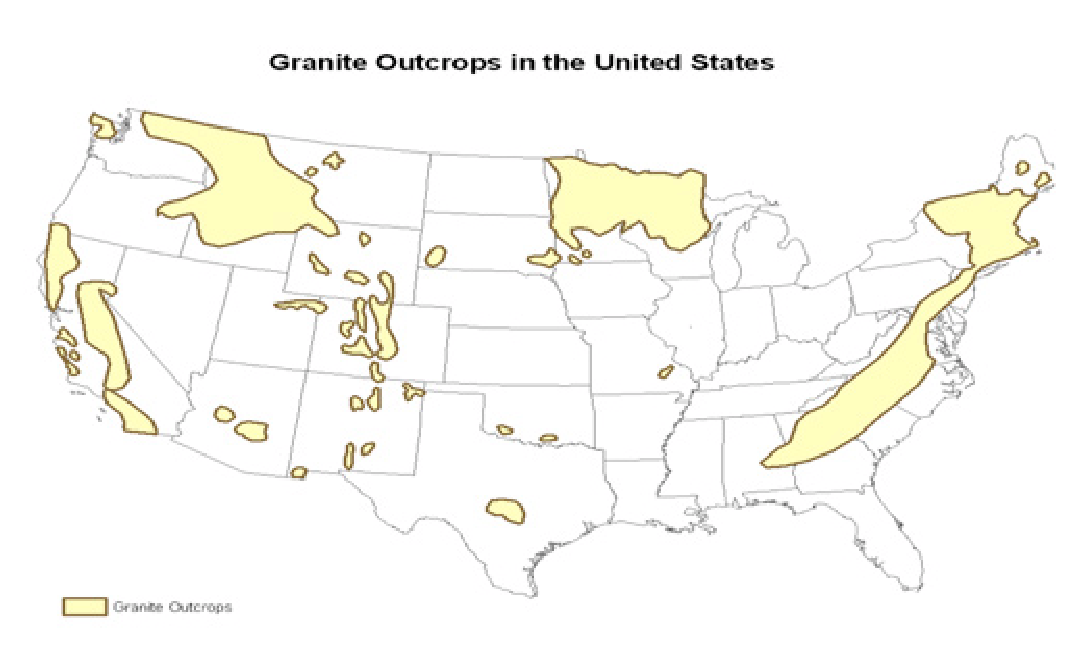
\includegraphics[width=0.8\textwidth]{./images/graniteBush.eps}
         \caption{U.S. Granite Beds, ref. \cite{bush_economic_1976}.}
     \end{figure}
   \end{minipage}
\end{frame}

\begin{frame}
  \frametitle{Clay Disposal Environments}
  \footnotesize{

  \begin{figure}[h!]
    \begin{center}
      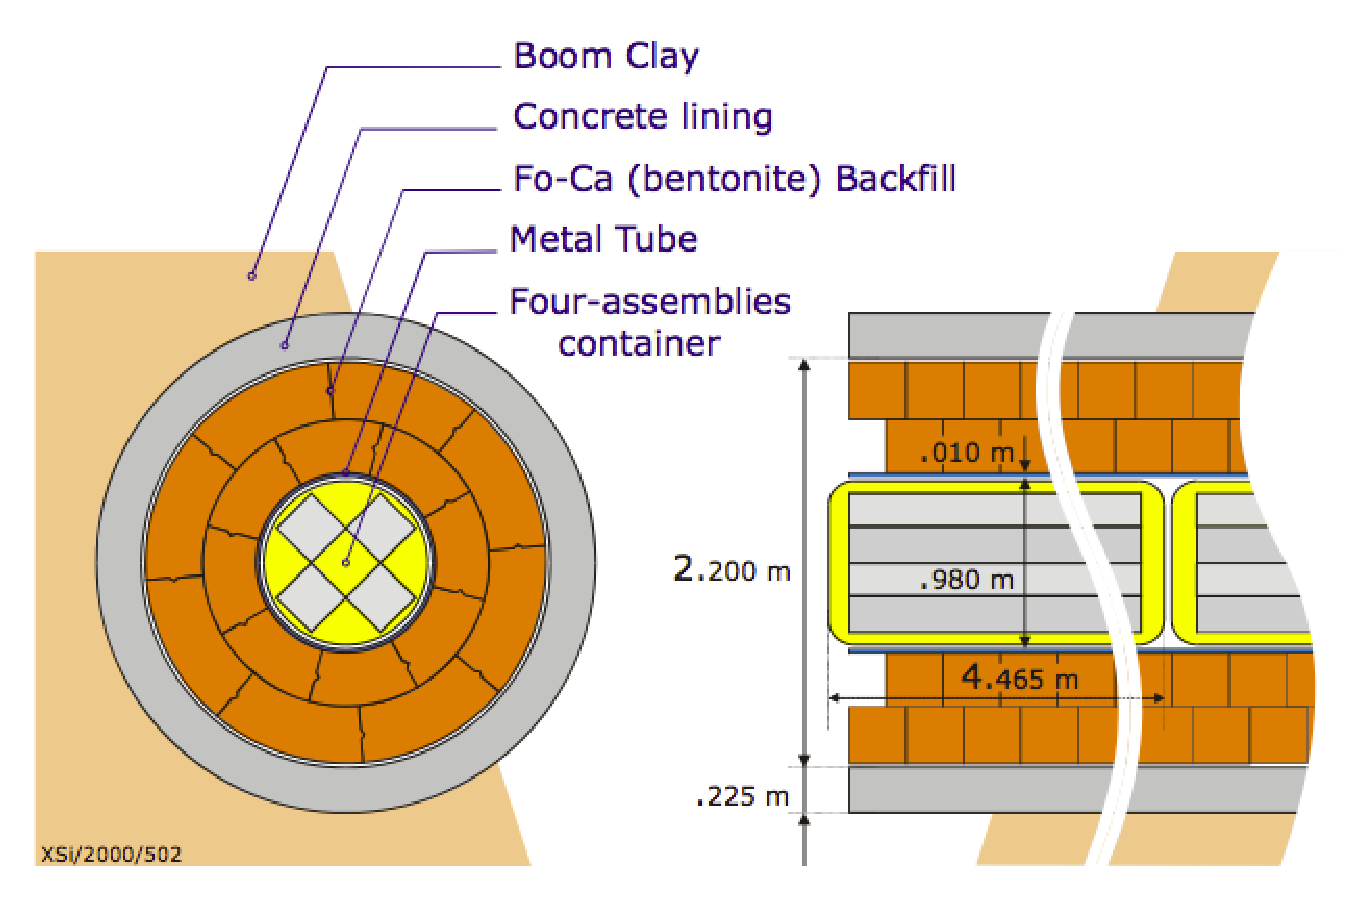
\includegraphics[height=.7\textheight]{./images/belgianClayRedImp.eps}
    \end{center}
    \caption{Belgian reference concept in Boom Clay 
    \cite{von_lensa_red-impact_2008}.}
    \label{fig:belgianClayRedImp}
  \end{figure}

}
\end{frame}

\begin{frame}
  \frametitle{Granite Disposal Environments}
  \footnotesize{

  \begin{figure}[h!]
    \begin{center}
      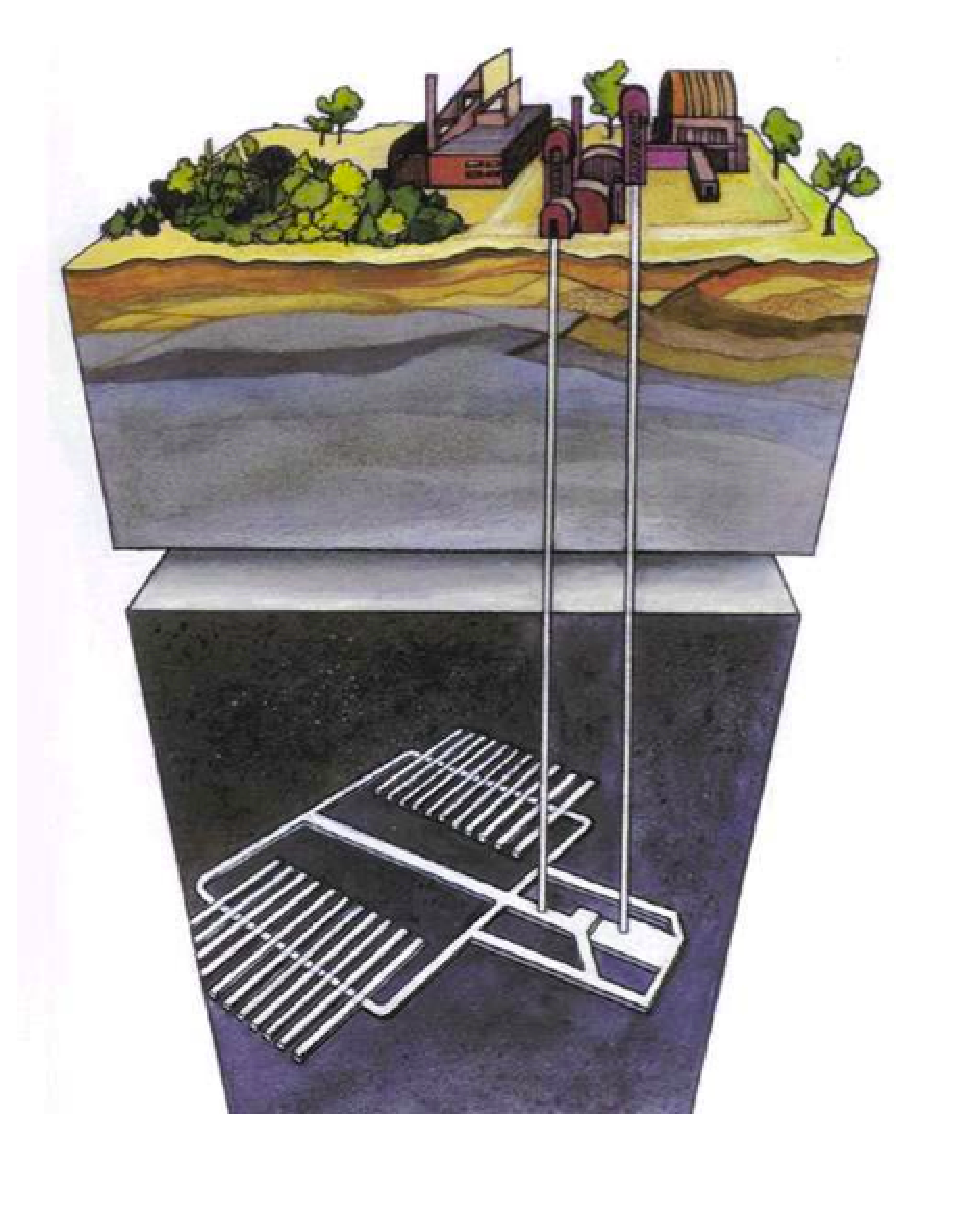
\includegraphics[height=.7\textheight]{./images/czechGraniteRedImp.eps}
    \end{center}
    \caption{Czech reference concept in Granite 
    \cite{von_lensa_red-impact_2008}.}
    \label{fig:czechGraniteRedImp}
  \end{figure}
}
\end{frame}

\begin{frame}
  \frametitle{Salt Disposal Environments}
  \footnotesize{

  \begin{figure}[h!]
    \begin{center}
      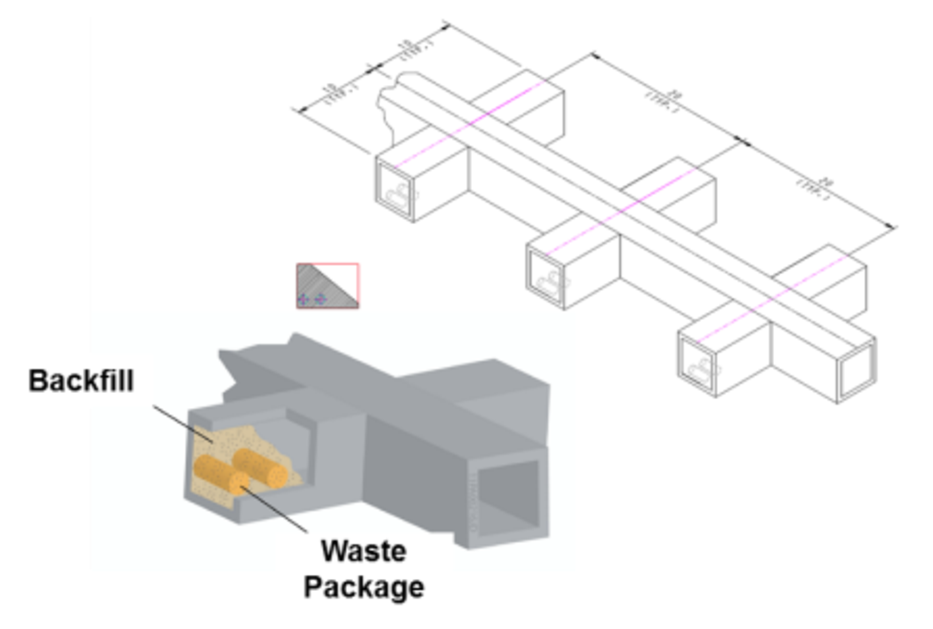
\includegraphics[height=.7\textheight]{./images/carter_salt_layout.eps}
    \end{center}
    \caption{DOE-NE Used Fuel Disposition Campaign  concept in 
    Salt \cite{hardin_generic_2011}.}
    \label{fig:salt_layout}
  \end{figure}
}
\end{frame}
\begin{frame}
  \frametitle{Salt Disposal Environments}
  \footnotesize{

  \begin{figure}[h!]
    \begin{center}
      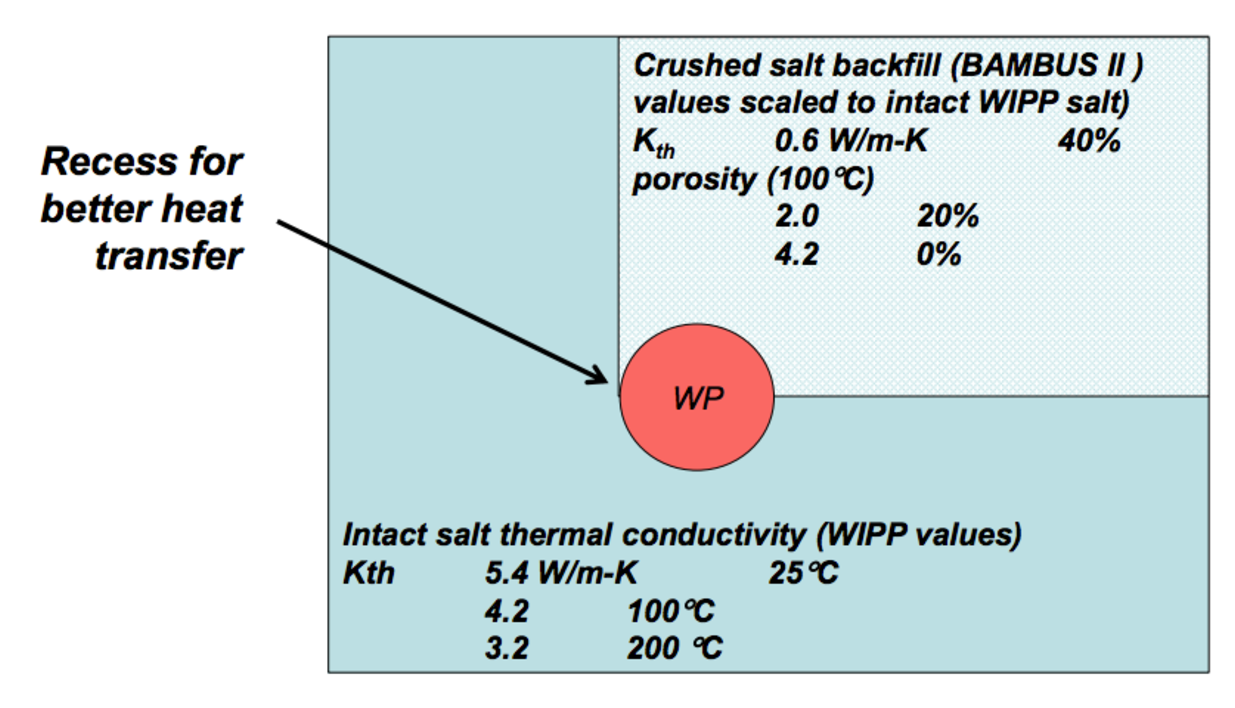
\includegraphics[height=.7\textheight]{./images/hardin_salt_layout.eps}
    \end{center}
    \caption{DOE-NE Used Fuel Disposition Campaign  concept in 
    Salt \cite{hardin_generic_2011}.}
    \label{fig:hardin_salt_layout}
  \end{figure}
}
\end{frame}

\begin{frame}
  \frametitle{Deep Borehole Disposal Environment}
  \footnotesize{

  \begin{figure}[h!]
    \begin{center}
      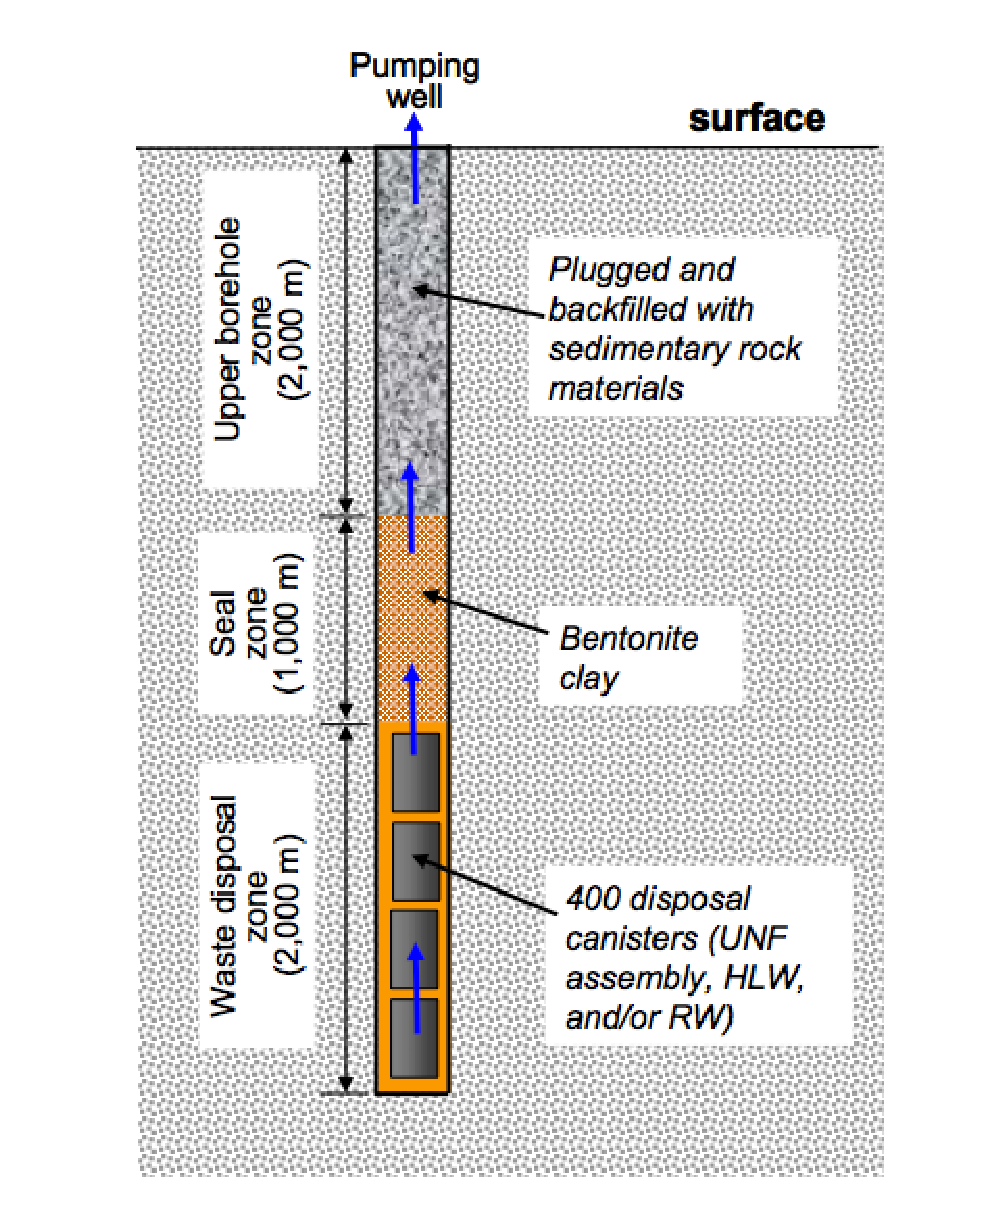
\includegraphics[height=.7\textheight]{./images/boreholeGPAM.eps}
    \end{center}
    \caption{DOE-NE Used Fuel Disposition Campaign Deep Borehole concept 
    \cite{hardin_generic_2011}.}
    \label{fig:boreholeGPAM}
  \end{figure}
}
\end{frame}




\section{Geologic Repository Performance}
\subsection{Metrics}

%%----------------------------------------%%
\begin{frame}
  \frametitle{Performance Metrics}
  \begin{itemize}
  \item Dose
  \item Environmental Release 
  \item Repository Footprint
  \item Cost
  \item ...
\end{itemize}
\end{frame}

\subsection{Thermal Loading}

%%----------------------------------------%%
\begin{frame}
  \frametitle{Thermal Capacity in Various Geologies}
\footnotesize{
  \begin{figure}[htbp!]
  \begin{center}
    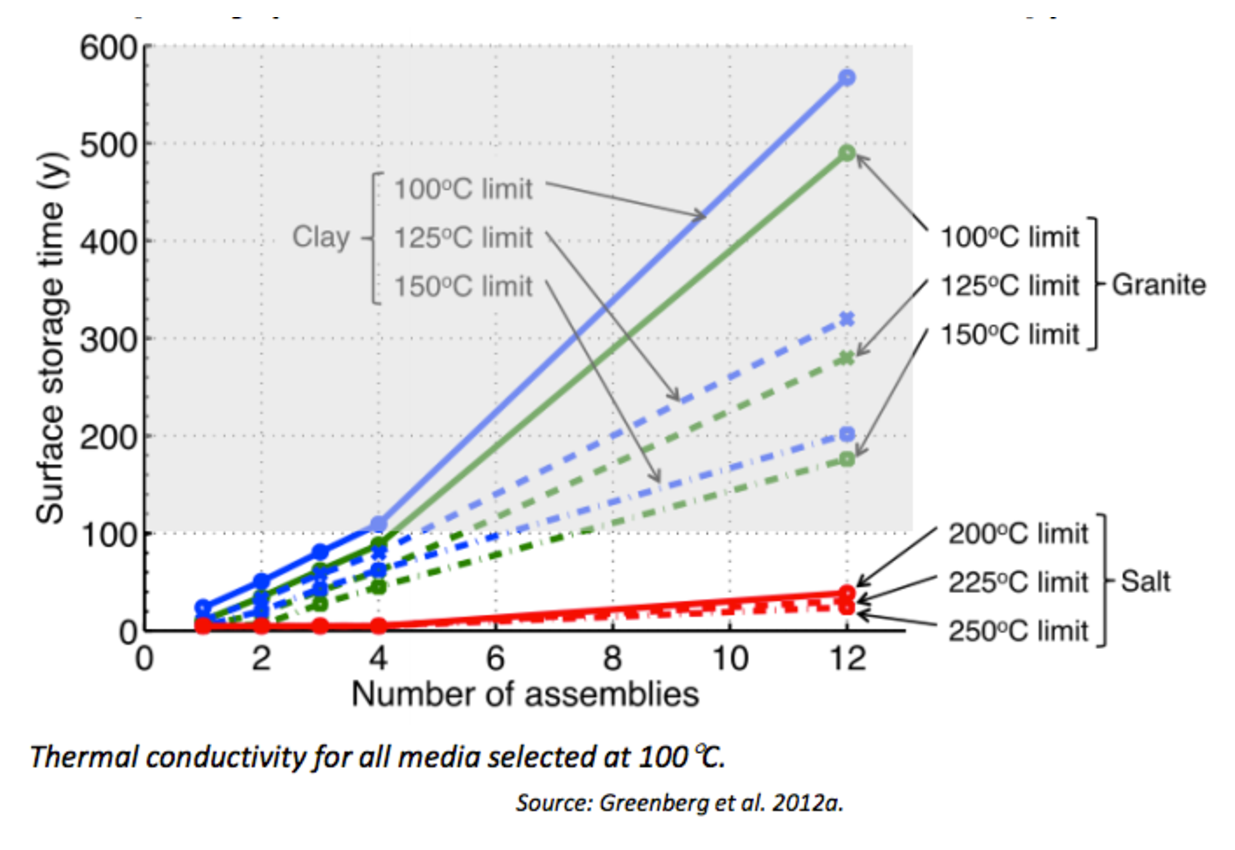
\includegraphics[width=0.7\textwidth]{./images/greenberg_thermal.eps}
  \end{center}
  \caption{The varying thermal limits, thermal conductivities, and thermal 
    diffusivities of various geologies result in differing heat capacities to 
    similar waste \cite{greenberg_application_2012}.}
  \label{fig:greenberg_thermal}
\end{figure}

}
\end{frame}

\subsection{Radionuclide Transport and Release}

%%----------------------------------------%%
\begin{frame}
  \frametitle{Release Mechanisms}
  \begin{itemize} 
  \item Human Disruption
  \item Natural Disruption
  \item Barrier Dissolution
  \item Advection
  \item Diffusion
  \item Sorption
  \item Solubility Limitation
  \item ... 
  \end{itemize}
\end{frame}

%%----------------------------------------%%
\begin{frame}
\frametitle{Solubility Sensitivity In A Clay Model}
\begin{figure}[ht]
  \centering
  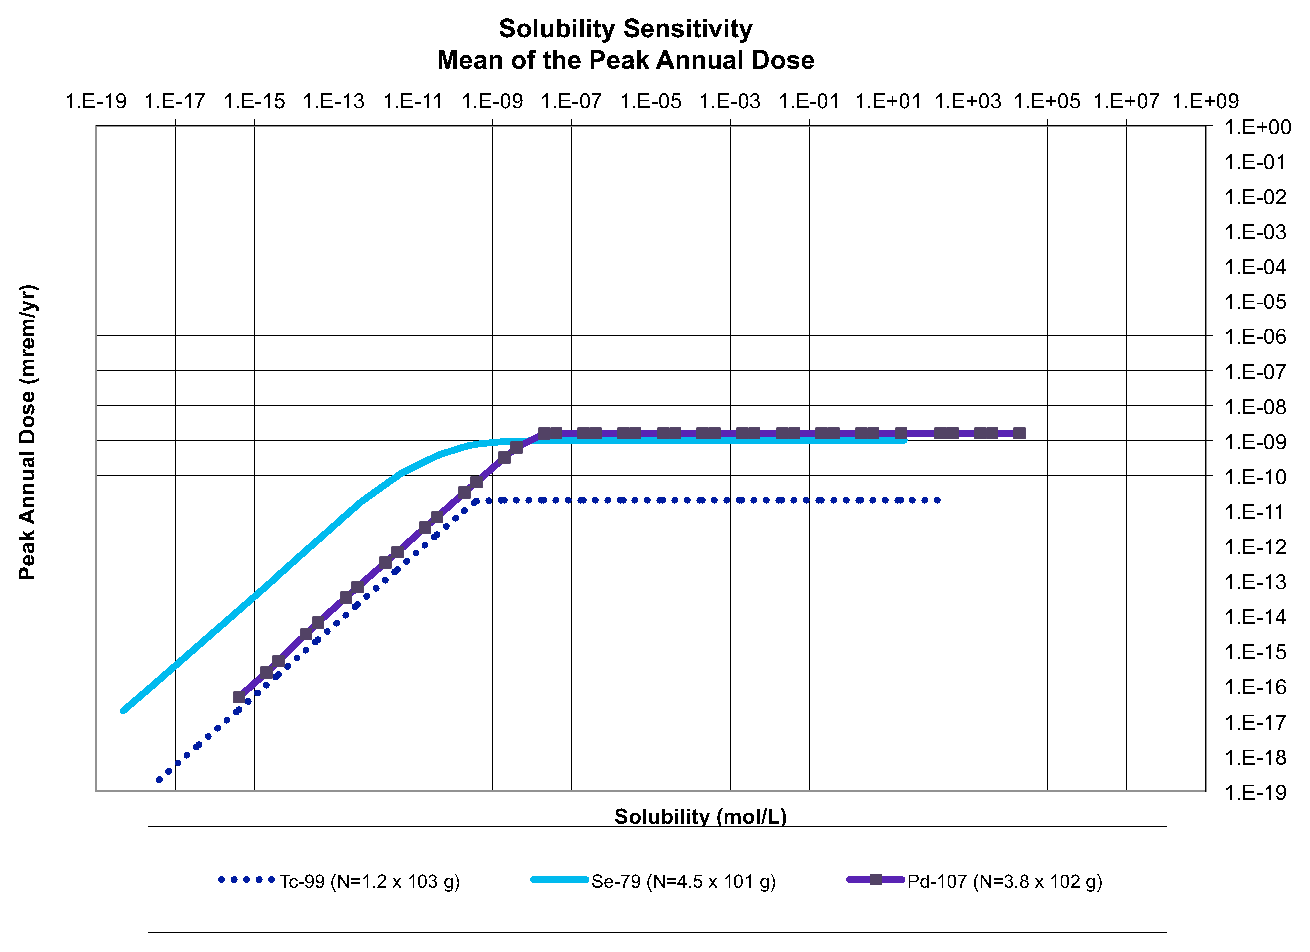
\includegraphics[width=0.7\linewidth]{./images/Solubility_Summary.eps}
  \caption{Solubility limit sensitivity. The peak annual dose due to an 
  inventory, $N$, of each isotope.}
  \label{fig:SolSum}
\end{figure}
\end{frame}

%%----------------------------------------%%
\begin{frame}
\frametitle{Retardation Sensitivity In A Clay Model}
\begin{figure}[ht]
  \centering
  \includegraphics[width=0.7\linewidth]{./images/Partitioning_Summary.eps}
  \caption{$K_d$ sensitivity.  The peak annual dose due to an inventory, 
  $N$, of each isotope.}
  \label{fig:KdSum}
\end{figure}
\end{frame}

%%----------------------------------------%%
\begin{frame}[c]
  \frametitle{Example : Vertical Advective Velocity and Diffusion Coefficient}
\begin{figure}[htp!]
\centering
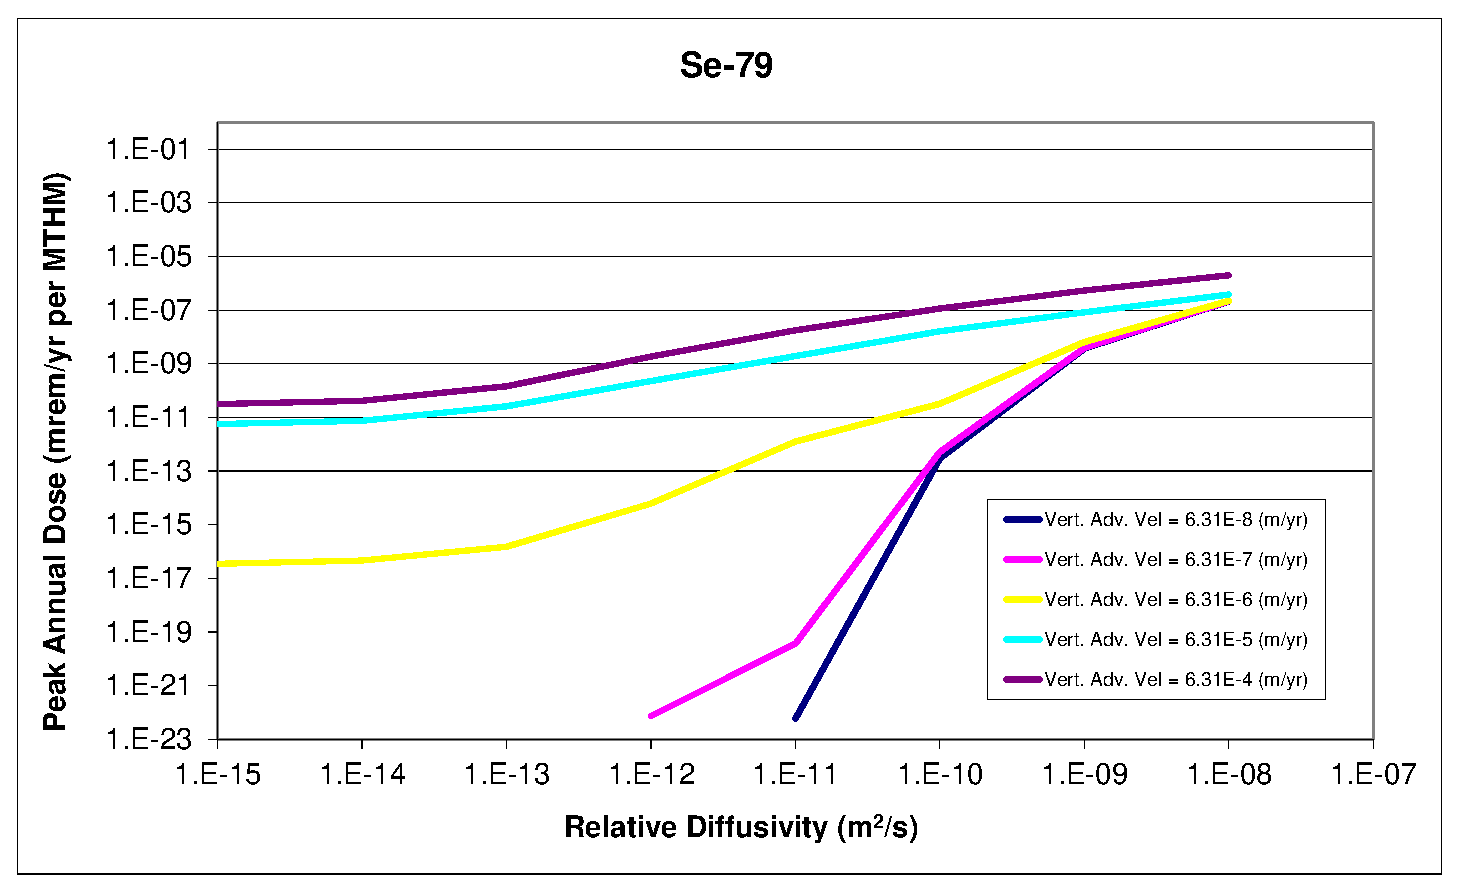
\includegraphics[width=0.8\textwidth]{./images/Se-79.eps}
\caption{$^{79}Se$.  $Se$ is non sorbing, but solubility limited in clay.  For low vertical advective velocity, the system is diffusion dominated.}
\label{fig:VAdvVelSe79}
\end{figure}
\end{frame}

%%----------------------------------------%%
\begin{frame}[c]
  \frametitle{Example : Vertical Advective Velocity and Diffusion Coefficient}
\begin{figure}[ht!]
\centering
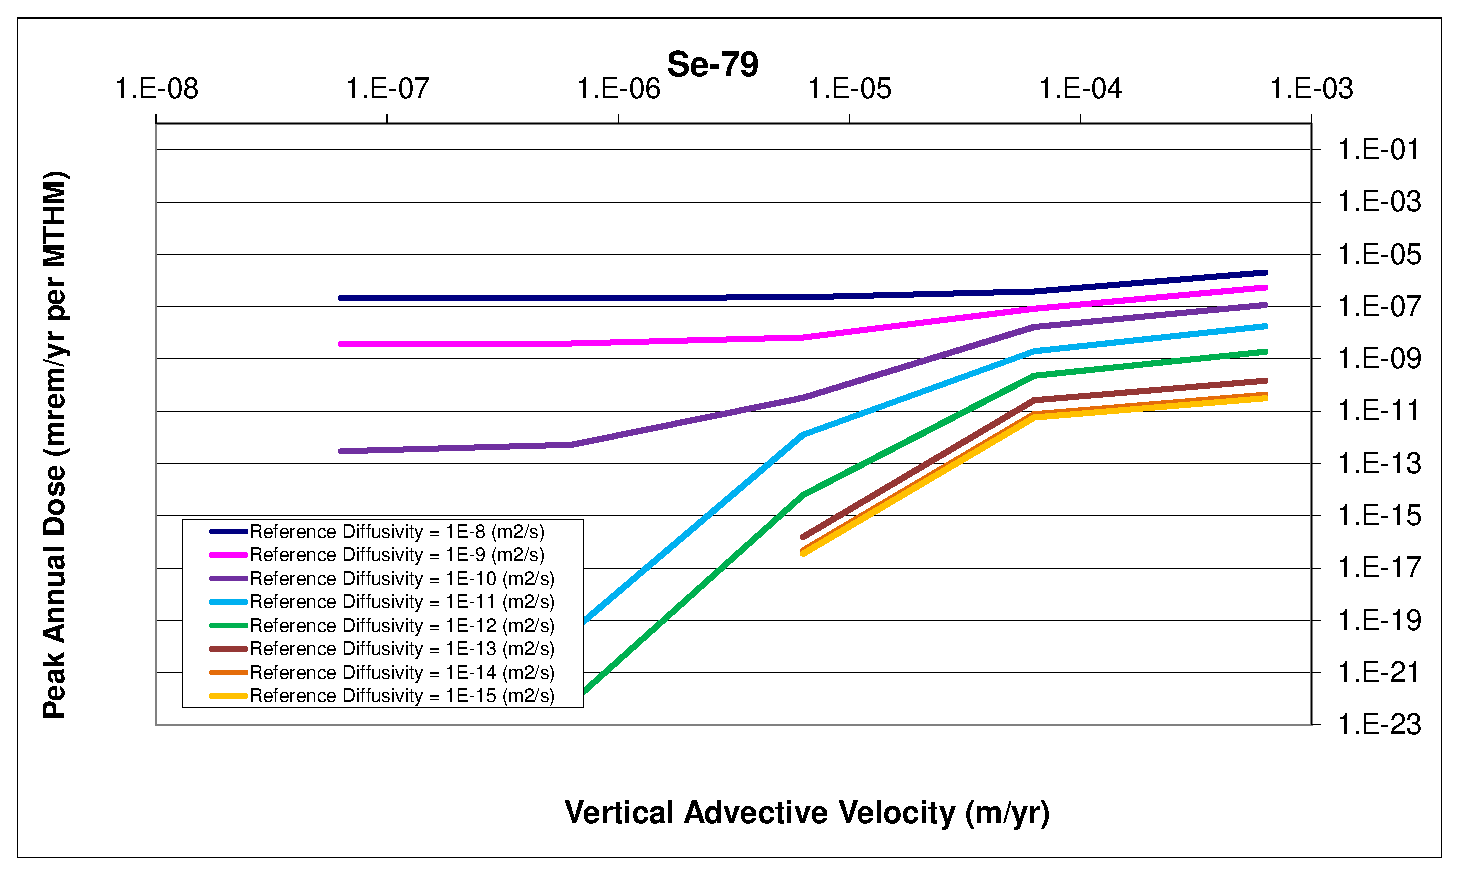
\includegraphics[width=0.8\textwidth]{./images/Se-79-VAdvVel.eps}
\caption{$^{79}Se$.
$Se$ is non sorbing, but solubility limited in clay.
For high vertical advective 
velocity, the diffusivity remains important even in the advective regime as 
spreading facilitates transport in the presence of solubility limited 
transport.} 
\label{fig:VAdvVelSe79VAdvVel}
\end{figure}
\end{frame}



\section{Fuel Cycle Impacts}
\subsection{Thermal Contributors}

%%----------------------------------------%%
\begin{frame}
  \frametitle{Heat Contributors In PWR SNF}
\footnotesize{
  \begin{figure}[htbp!]
  \begin{center}
    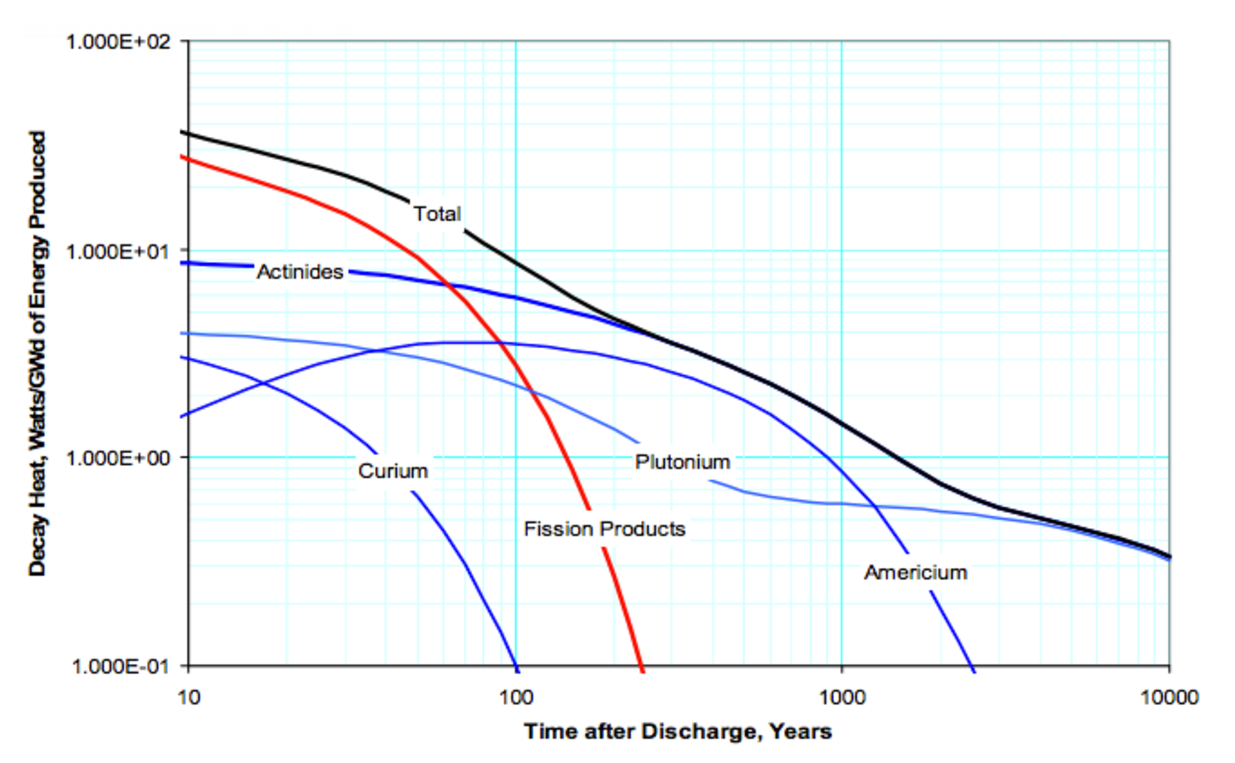
\includegraphics[width=0.7\textwidth]{./images/wigeland_heat.eps}
  \end{center}
  \caption{Heat contributors in a canonical PWR 
    fuel\cite{wigeland_relationship_2010}.}
  \label{fig:<++>}
\end{figure}

}
\end{frame}

%%----------------------------------------%%
\begin{frame}
  \frametitle{Heat Contributors in PWR SNF}
\footnotesize{
  \begin{figure}[htbp!]
  \begin{center}
    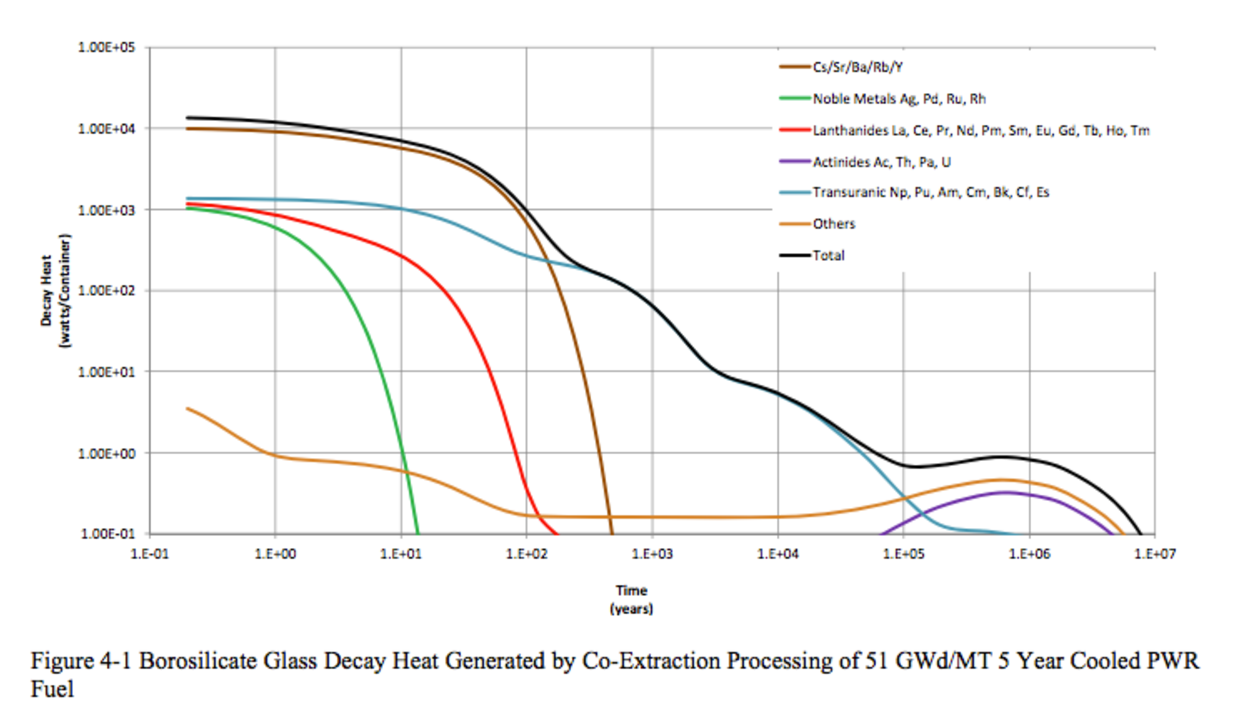
\includegraphics[width=0.7\textwidth]{./images/carter_coex_heat.eps}
  \end{center}
  \caption{Heat contributors in the primary result of a once through PWR fuel 
    cycle \cite{carter_us_2011}.}
  \label{fig:carter_coex_heat}
\end{figure}

}
\end{frame}
%%----------------------------------------%%
\begin{frame}
  \frametitle{Heat Contributors in LWR Recycled MOX}
\footnotesize{
  \begin{figure}[htbp!]
  \begin{center}
    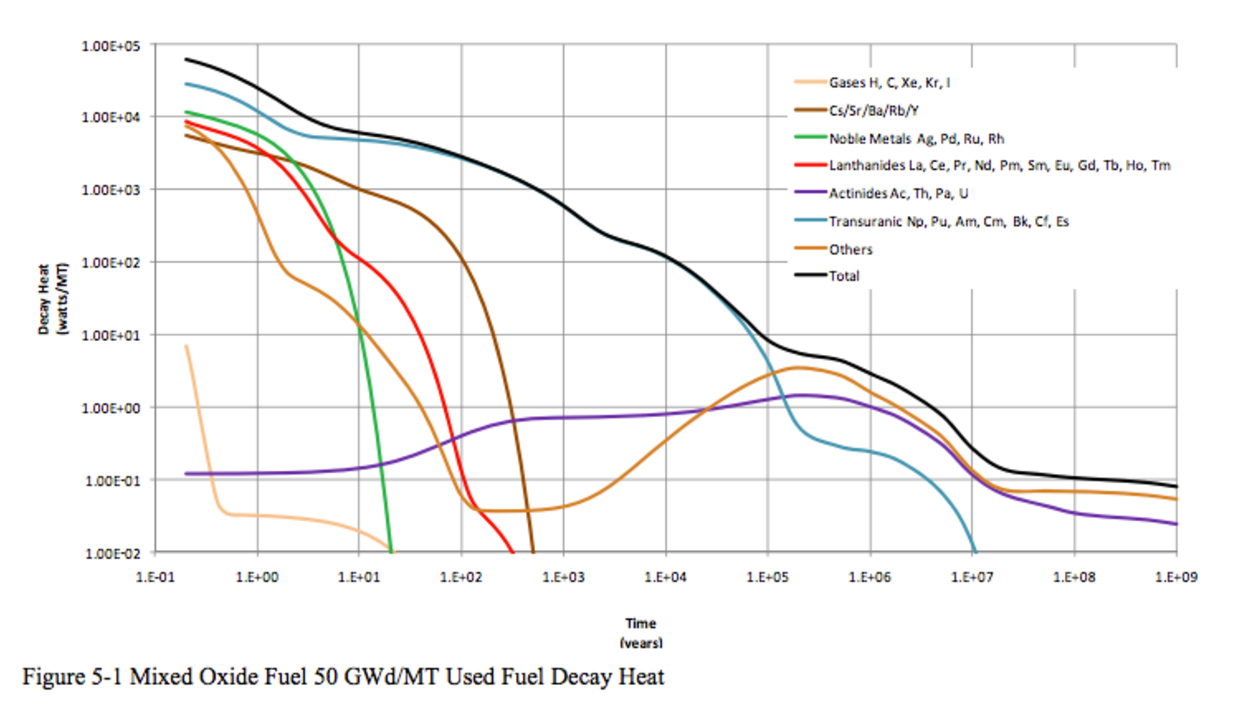
\includegraphics[width=0.7\textwidth]{./images/carter_lwr_mox_heat.eps}
  \end{center}
  \caption{Heat contributors in the primary result of MOX recycling in an LWR
    \cite{carter_us_2011}.}
  \label{fig:carter_lwr_mox_heat}
\end{figure}

}
\end{frame}
%%----------------------------------------%%
\begin{frame}
  \frametitle{Heat Contributors After NUEX Recycling}
\footnotesize{
  \begin{figure}[htbp!]
  \begin{center}
    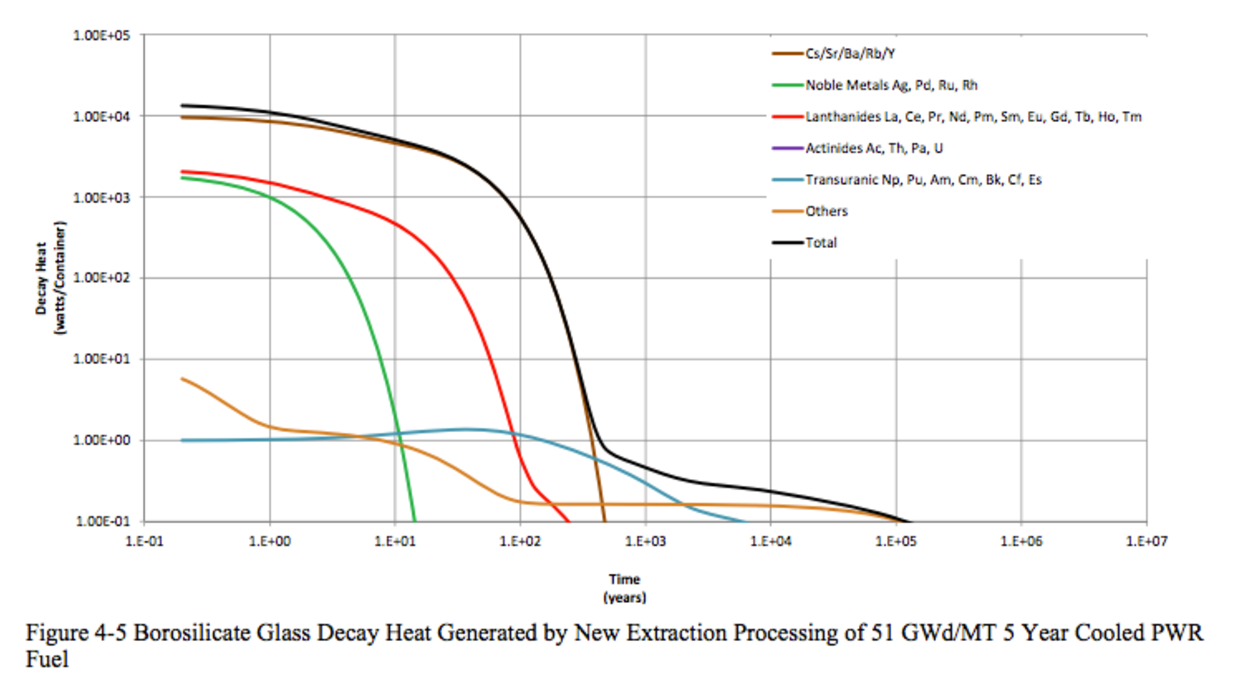
\includegraphics[width=0.7\textwidth]{./images/carter_nuex_heat.eps}
  \end{center}
  \caption{Heat contributors in the primary result of the NUEX extraction 
    process\cite{carter_us_2011}.}
  \label{fig:carter_nuex_heat}
\end{figure}

}
\end{frame}

%%----------------------------------------%%
\begin{frame}
  \frametitle{Heat Contributors After COEX Recycling}
\footnotesize{
  \begin{figure}[htbp!]
  \begin{center}
    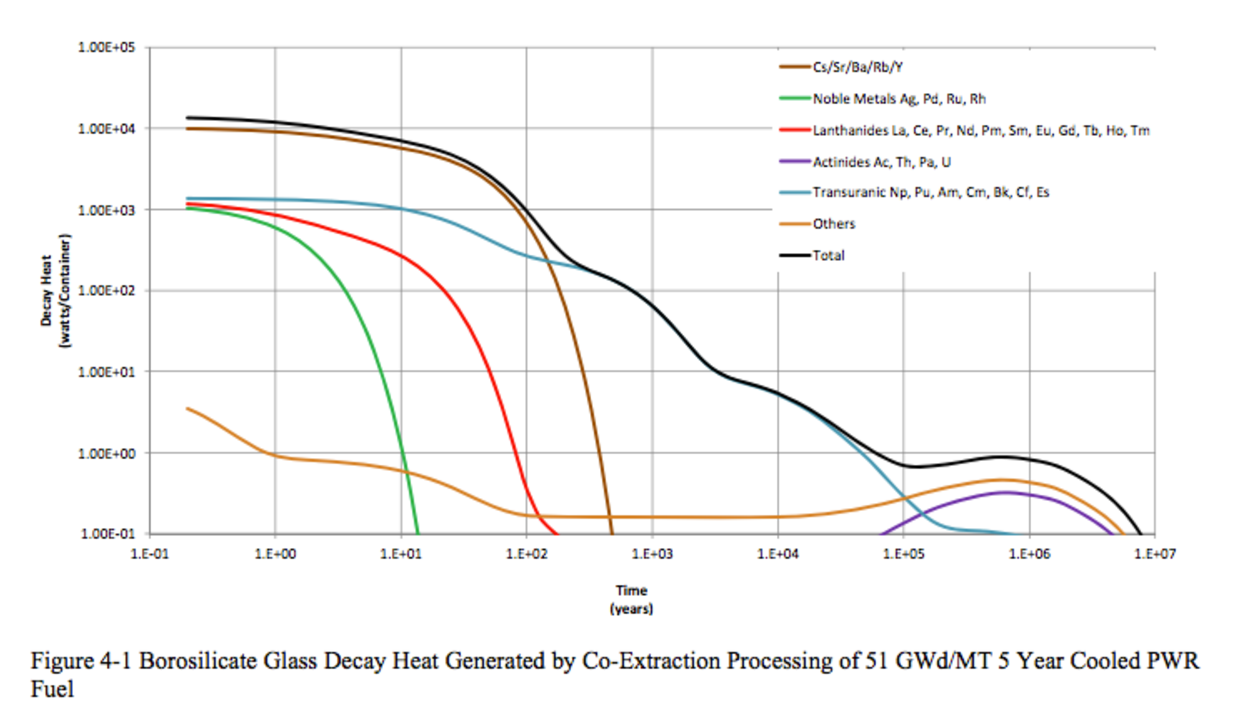
\includegraphics[width=0.7\textwidth]{./images/carter_coex_heat.eps}
  \end{center}
  \caption{Heat contributors in the primary result of the COEX extraction 
    process\cite{carter_us_2011}.}
  \label{fig:carter_coex_heat}
\end{figure}

}
\end{frame}
%%----------------------------------------%%
\begin{frame}
  \frametitle{Summary: Heat Contributing Isotopes in Various Fuel Cycles}
Dominant thermal contributors vary among fuel cycles. 
\begin{itemize}
   \item Recycling schemes are likely to reduce transuranics and actinides.
   \item Fission products such as Cs and Sr are powerful heat contributors in 
     the first 500 years, when capacity limiting peak heat is likely to occur in 
     many geologies.
   \item Transuranics, Pu, Np, Am, and Cm are dominant long term heat contributors. Some extraction processes are more successful at removing those from the waste stream. 
\end{itemize}
\end{frame}

\subsection{Dose Contributors}

%%----------------------------------------%%
\begin{frame}
  \frametitle{Dose Contributors, PWR SNF In Yucca}
\footnotesize{
  \begin{figure}[htbp!]
  \begin{center}
    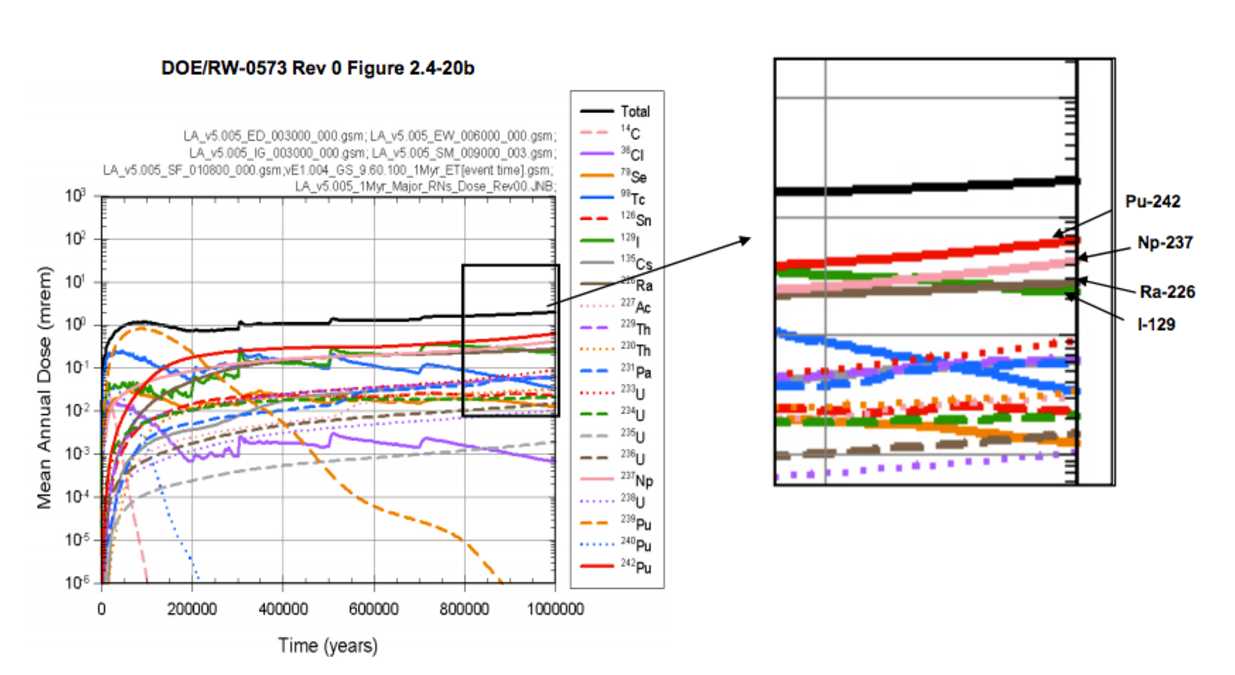
\includegraphics[width=0.7\textwidth]{./images/swift_dose_yucca.eps}
  \end{center}
  \caption{Dose contributors expected in the Yucca Mountain repository 
    \cite{swift_applying_2010}. In the oxidizing environment at Yucca mountain, 
    actinides such as $^{242}Pu$ and $^{237}Np$ dominate dose contribution. We 
    also see that long-lived, highly soluble $^{129}I$ and highly soluble 
    $^{226}Ra$ are also primary dose contributors.}
  \label{fig:swift_dose_yucca}
\end{figure}

}
\end{frame}

%%----------------------------------------%%
\begin{frame}
  \frametitle{Dose Contributors, PWR SNF In Clay}
\footnotesize{
  \begin{figure}[htbp!]
  \begin{center}
    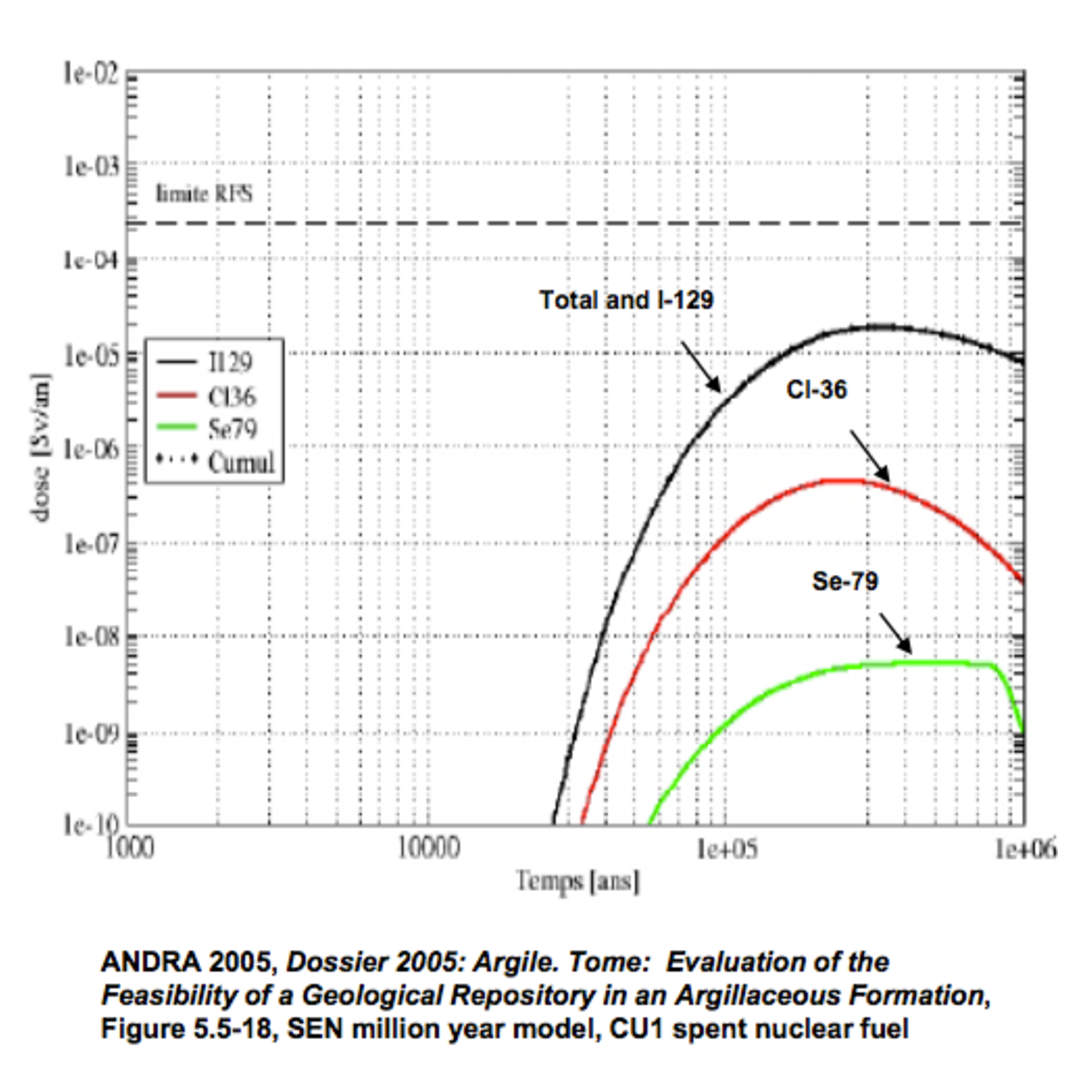
\includegraphics[width=0.5\textwidth]{./images/swift_clay_dose.eps}
  \end{center}
  \caption{Dose contributors expected in a clay repository concept 
    \cite{swift_applying_2010}. Primary contributors are highly soluble, long 
    lived isotopes $^{129}I$, $^{36}Cl$, and $^{79}Se$ .}
  \label{fig:swift_clay_dose}
\end{figure}

}
\end{frame}

%%----------------------------------------%%
\begin{frame}
  \frametitle{Dose Contributors, PWR SNF In Granite}
\footnotesize{
  \begin{figure}[htbp!]
  \begin{center}
    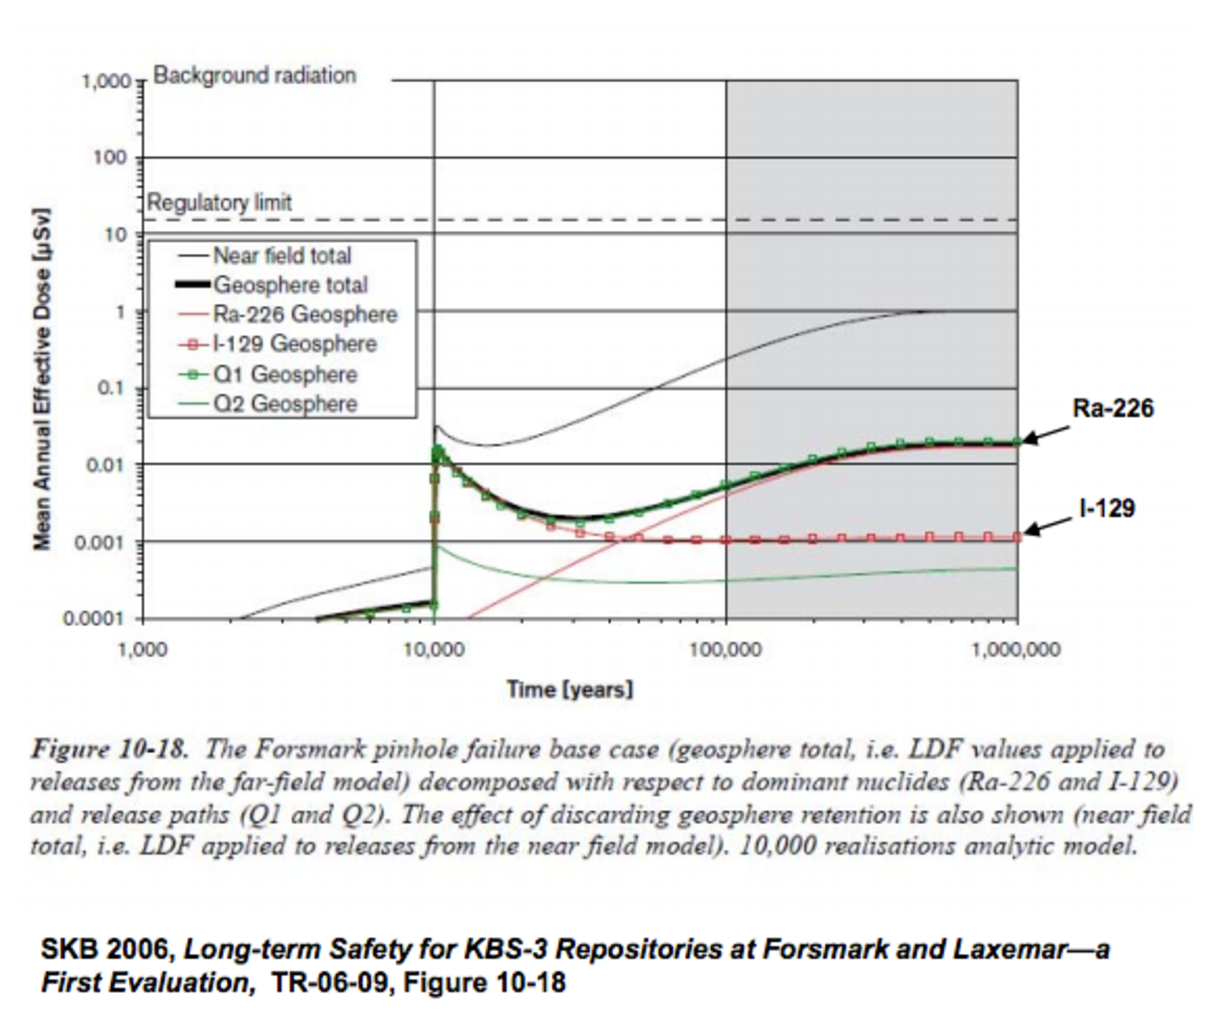
\includegraphics[width=0.7\textwidth]{./images/swift_granite_dose.eps}
  \end{center}
  \caption{Dose contributors expected in a granite repository concept 
    \cite{swift_applying_2010}. Primary contributors in this more advective 
  system are the most mobile products at the time of waste package failure. 
  $^{129}I$ is always a primary contributor.}
  \label{fig:swift_granite_dose}
\end{figure}

}
\end{frame}

%%----------------------------------------%%
\begin{frame}
  \frametitle{Summary: Dose Contributing Isotopes in Various Geologies}
Dominant dose contributors vary among geologies due to both \textbf{water chemistry (sorption, solubility)} and \textbf{transport regime (diffusive, advective)}. 
\begin{itemize}
  \item Long lived, highly soluble, non sorbing $^{129}I$ is a dominant long-term
contributor in all geologies.
  \item In a tuff geology like Yucca Mountain, which is oxidizing with advective transport, actinides dominate in addition to $^{129}I$.
  \item In granite, a typically reducing geology with advective release pathways, mobile $^{226}Ra$ may be important in addition to $^{129}I$.
  \item In primarily diffusive salt and clay geologies, long-lived, highly soluble, non-sorbing fission and activation products ($^{129}I$, $^{36}Cl$, $^{79}Se$)  dominate. 
\end{itemize}
\end{frame}

\subsection{Other Factors}

%%----------------------------------------%%
\begin{frame}
  \frametitle{Volume}
\footnotesize{
  \begin{figure}[htbp!]
  \begin{center}
    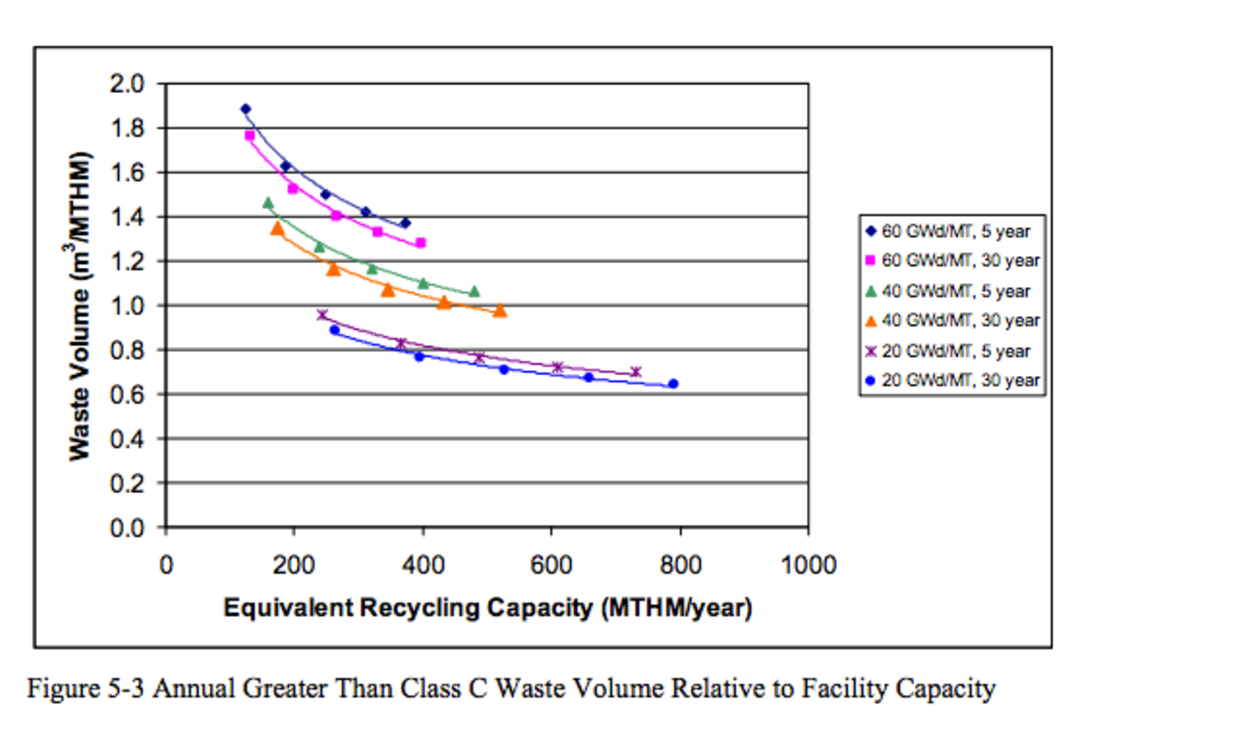
\includegraphics[width=0.7\textwidth]{./images/carter_volume.eps}
  \end{center}
  \caption{Recycling strongly affects high level waste volumes\cite{carter_us_2011}.}
  \label{fig:carter_volume}
\end{figure}

}
\end{frame}



%%----------------------------------------%%
\begin{frame}
  \frametitle{Conclusion}
  Thanks!
  
  Feel free to direct questions to kdhuff@illinois.edu.
\end{frame}

%%--------------------------------%%
%%--------------------------------%%
\begin{frame}[allowframebreaks]
  \frametitle{References}
  \bibliographystyle{plain}
  {\footnotesize \bibliography{ne571} }

\end{frame}

%%--------------------------------%%




\end{document}



